\section{Introduction}
\label{sec:intro}

Retail decisions run at different grains and on different clocks. Supplier
range, space and cost reviews look at an item's volume across the chain over 26
or 52 weeks, and the terms agreed in them commit allowances for the year ahead.
Promotions are planned item by week in blocks of six to twelve weeks, and the
promotional and retail allowances that fund them follow the same blocks.
Merchants judge their category week by week. Store inventory is ordered item by
store, day by day \cite{fildes2022}. Each of these decisions reads the same
demand at a different grain and over a different span of time.

Since there is no single grain, there is no reason to expect one model to be
the most accurate at every grain and every horizon. Retailers do not want a
separate model at each grain either. Separate models disagree, and value leaks
at each hand-off from a coarse long-range plan to a finer short-range one. The
annual plan agreed with a supplier is broken into promotion blocks, weeks and
store orders. Where the finer forecasts do not add back to the plan, the gap is
paid for in stock, markdowns or lost sales. The forecasting literature treats
this as coherence across the levels of the product and store hierarchy
\cite{hyndman2011,mint} and across levels of time \cite{athanasopoulos2017},
usually by forecasting each level and reconciling the forecasts. This paper
takes the other route retailers use: one forecast made at the finest grain,
item by store by period, and summed to every coarser grain, so that the grains
add up by construction. The question this paper answers is whether one
forecast, built once at the finest grain, can serve the decisions a retailer
makes from it, across every kind of line, and which kind of model, or
combination of models, does that best.

Lines differ as much as grains do. In grocery a short head of fast lines
carries most of the units, and a long tail of slow lines sells a few units a
week or none. On the Dominick's categories studied here, \rqFastShareDomLo{}
to \rqFastShareDomHi{}\% of the items make 80\% of unit sales. Ranges also
change: items are added and delisted and stores open, so part of every forecast
is for a line or a store with little or no history. A forecast that serves the
fast lines well can fail on the tail or on a new item, and a planner deciding
for one kind of line needs to know which.

We test four kinds of model. Gradient-boosted trees are the proven method:
LightGBM was behind the leading entries of the M5 competition
\cite{m5accuracy}. Pretrained foundation models (TimesFM, Chronos-Bolt and
Timestral) forecast without training on the retailer's data. The Temporal
Fusion Transformer is an attention-based model trained on it. World models, the
newest of the four, learn a state for each item and carry it forward one period
at a time under the price and promotion plan; ours is shown in
Figure~\ref{fig:overview}. The world model and LightGBM were each tuned by the
same search on every data set, and the average of forecasts is tested
alongside them. The data are four public data sets: M5, six categories of
Dominick's, Breakfast at the Frat, and Corporaci\'on Favorita.

The study covers the short end of the planning cycle. Forecasts run 8 weeks
ahead on the weekly data and 28 days ahead on the daily data, and are scored at
every grain from item by store to the chain total, period by period and summed
over the whole window as a promotion block. Forecasts of 26 or 52 weeks are not
tested: judging them needs a retailer's own plans and range decisions to score
against, which no public data set carries, and is left for work with an
industry partner. Of the four Ps of retail, the study covers price and
promotion, through the plan inputs these data record; product and place are out
of scope. Every analysis was written down before it ran; the few added after
the first results were read are listed in Section~\ref{sec:limits}.

Section~\ref{sec:framework} sets out the framework, and the results follow it
part by part: grain, the nature of the line, seen and unseen data, and
transferability, with the broad view last.

\begin{figure*}[t]
\centering
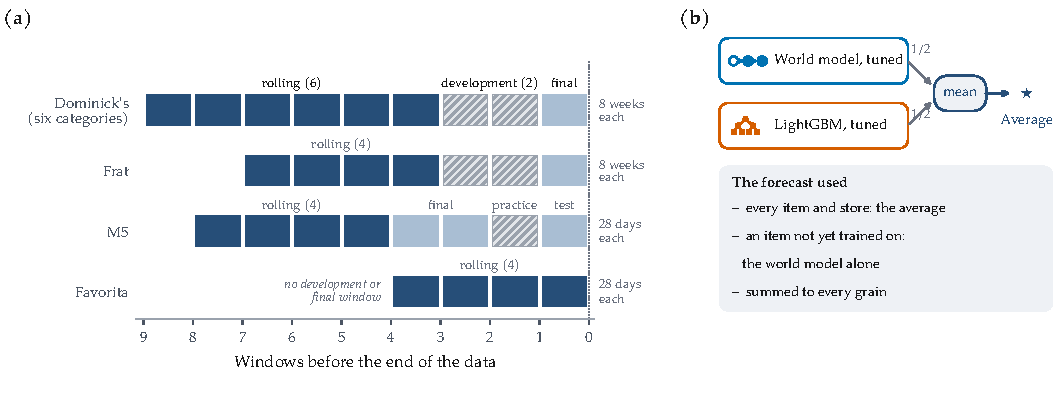
\includegraphics[width=\textwidth]{figs/fig_study.pdf}
\caption{\textbf{Every result of Section~\ref{sec:results} is scored on rolling
windows that no choice of setting saw, and the forecast recommended is the average of the two tuned
models.} \textbf{(a)} Windows by data set, in windows before the end of the data:
the rolling windows scored in this paper; and the development and final windows
of the first version, which are not scored here. The searches that tuned each
model scored windows earlier than the rolling windows. \textbf{(b)} The forecast
that the results support: the equal-weight average of the tuned world model and
the tuned LightGBM for every item and store, the world model alone for an item
the models have not yet been trained on, summed to every grain.}
\label{fig:study}
\end{figure*}

\begin{figure*}[t]
\centering
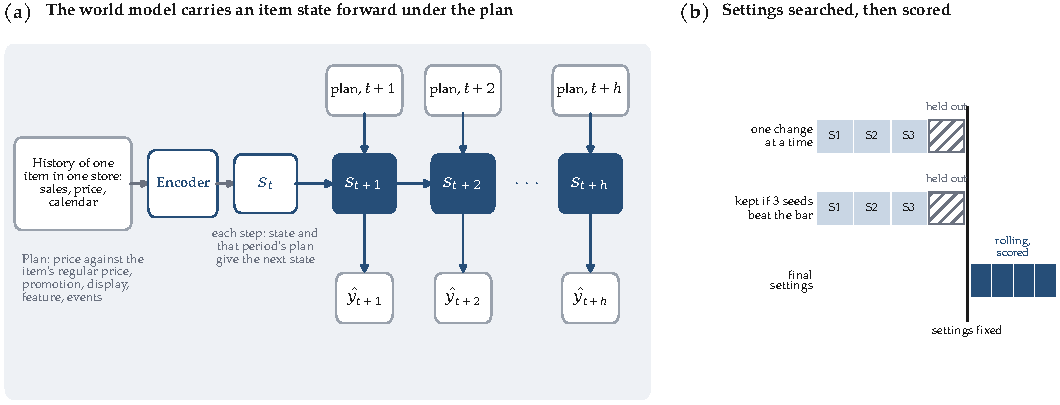
\includegraphics[width=\textwidth]{figs/fig_overview.pdf}
\caption{\textbf{The world model carries each item's state forward under the
plan.} \textbf{(a)} An encoder turns the recent history of one item in one store into
a state $s_t$. A transition step takes the state and one period's plan and
gives the state one period later; each period's sales are read from the state
as it stands after the plan so far. \textbf{(b)} Each model's settings were
searched one change at a time on early windows (S1 to S3), a change kept only if
its mean over three seeds beat the best so far by the keep bar, with the latest
search window held out of every decision; the final settings were then scored
once on the later rolling windows (Section~\ref{sec:loop}).}
\label{fig:overview}
\end{figure*}

Section~\ref{sec:related} places the work among retail promotion models,
hierarchical evaluation, forecast combination, pretrained forecasters and world
models. Sections~\ref{sec:data} to \ref{sec:setup} give the data, the models and
the experimental setup. Section~\ref{sec:results} reports the results,
Section~\ref{sec:dropped} what was tried and dropped\ifjournal{} (in the online
supplement, with the supporting analyses and the detail of the searches)\fi, and
Sections~\ref{sec:discussion} to \ref{sec:conclusion} discuss what the results
mean for a retailer, their limits, and conclude.

% =====================================================================
\section{Framework}
\label{sec:framework}

The overall question of this paper is:

\begin{quote}
Can one forecast, built once at the finest grain of item by store by period and
summed to every coarser grain, serve the decisions a retailer makes from it
across every kind of line, and which kind of model, or combination of models,
does that best?
\end{quote}

\noindent It is answered through four research questions, in the order a
retailer meets them:

\begin{description}\setlength{\itemsep}{2pt}
\item[RQ1, grain.] At which grains of product, store and time does each model
  forecast best, period by period and over a whole promotion block, when every
  grain is summed from the same item-by-store forecast?
\item[RQ2, nature of the line.] How does each model do on the fast lines that
  carry most of the sales, on the long tail of slow lines, and on lines with
  short history?
\item[RQ3, seen and unseen data.] How much accuracy does each model lose on
  items and stores it was not trained on?
\item[RQ4, transferability.] Do a model's settings carry to another retailer,
  and does training on other retailers' data make it more accurate?
\end{description}

\noindent These are the questions retailers ask of a forecast in practice
(Section~\ref{sec:background}). Each question fixes what is measured before any
model is compared,
and the results are reported in the same order (Section~\ref{sec:results}).
The broad view then brings the four answers together.

\paragraph{RQ1, grain} Does the forecast hold up at every grain a decision is made
at, and do the grains add up? Every model forecasts each item in each store for
each period, and the forecasts are summed to item, store, category, category by
store and the chain total. Each grain is scored period by period, which is how
store orders and the category week are judged, and over the whole forecast
window as one block, which is how a promotion is judged. Because every grain is
a sum of the same item-by-store forecast, the plans built from them add up, and
any value lost between grains shows as a difference in accuracy between them.

\paragraph{RQ2, nature of the line} Does the forecast hold up on every kind of
line? Grocery sales are concentrated: a short head of fast lines carries most of
the units, and a long tail of slow lines sells a few units a week or none. Lines
also differ in how much history they have. The fast lines are defined as the
items that together make 80\% of unit sales over the year before the forecast,
the slow lines as the rest, and lines with short history as those whose first
sale falls less than 26 weeks before the forecast. Each part is scored on its
own series at every grain, so that the total of the fast lines, the slow lines
of each store, and so on, are each judged as a planner would judge them. The
share of items that makes 80\% of sales is reported for each data set.

\paragraph{RQ3, seen and unseen data} Does the forecast hold up on items and stores
the model was not trained on? Ranges change and stores open, so part of every
forecast is for lines or stores with little or no history in the model. A fifth
of the items, or of the stores, is kept out of training; once trained, each
model reads the kept-out series' recent sales and forecasts them. The cost of
not having trained on them is the accuracy lost on that fifth against a model
trained on everything.

\paragraph{RQ4, transferability} Do the settings carry to another retailer, and does
training on other retailers' data help? Settings tuned on M5 are carried
unchanged to Favorita and compared with settings tuned on Favorita itself. Each
model is also trained on its data set together with the other data sets, and
compared with the same model trained on its own data alone.

\paragraph{The broad view} The four parts are then brought together: which
model, or combination, gives the best balance across grains, lines and seen and
unseen data, and where each kind of model fits in the planning cycle. Findings
are reported for each grain and each kind of line, since that is what a
retailer needs to choose a model for a decision; the broad view simplifies them
and does not replace them.

% =====================================================================
\section{Related work}
\label{sec:related}

\subsection{Retail forecasting and the promotion plan}

Fildes, Ma and Kolassa~\cite{fildes2022} review retail forecasting research and
practice and note that most studies forecast and evaluate at one level of
aggregation, usually the item, although retail decisions are spread across
levels. Sales of a single item in a single store are intermittent, which led to
dedicated methods for intermittent demand~\cite{croston,syntetos2005} and to
evaluating forecasts as count distributions~\cite{kolassa2016}. The Tweedie
family~\cite{jorgensen1987}, a compound Poisson--gamma distribution with a point
mass at zero, is the loss many M5 entries used, and the loss we use.

Promotions move retail sales more than anything else in the plan. PromoCast
forecast promoted-week sales for a chain from the planned event and the item's
past response~\cite{promocast}. Van Heerde, Leeflang and
Wittink~\cite{vanheerde2000} and Mac\'e and Neslin~\cite{mace2004} measured
the dips in sales before and after a promotion, when shoppers stock up and then
buy less. Ma, Fildes and Huang~\cite{ma2016} showed that promotional information
from within and across categories improves item-level forecasts.
Gupta~\cite{gupta1988} split the promotion bump into brand switching, purchase
timing and quantity, and van Heerde, Gupta and Wittink~\cite{vanheerde2003}
showed that in units only about a third of the bump is switching from other
brands. Attraction models make an item's sales the category's sales times its
share~\cite{bell1975,cooper1988}; our brand-switching step follows that
structure. Dominick's Finer Foods ran pricing experiments across its
stores~\cite{hoch1995}, and its scanner data are behind much of this
work~\cite{dominicks}.

\subsection{Decisions across grains and lines}

Retail decisions read the same demand at different grains and over different
spans: replenishment item by store by day, promotions item by week, category
reviews by week, and range, space and supplier terms over a year or more
\cite{fildes2022}. Forecasts made separately for each grain need not agree, and
the literature restores agreement by reconciliation, across the product and store
hierarchy \cite{hyndman2011,mint}, across levels of time
\cite{athanasopoulos2017}, and across both together
\cite{kourentzes2019crosstemporal}. The alternative studied here, a single
forecast at the finest grain summed upward, is coherent by construction and is
the way the M5 competition scored its entries \cite{m5accuracy}; its cost is
that one model must serve every grain.

Lines also differ in how much they sell and how much history they have. A small
share of items carries most of the units, and the long tail sells a few units a
week or none, which led to dedicated methods for intermittent demand
\cite{croston,syntetos2005}. Lines with little or no history are forecast from
the histories of similar products: by matching a new product to the life-cycle
curves of earlier ones \cite{hu2019newproduct}, or from product attributes
\cite{vansteenbergen2020}. Global models trained across many series
\cite{montero2021} can forecast a series they were not trained on from its
recent sales alone, which is how the models in this study meet new items and
new stores.

\subsection{Hierarchies, combinations and evaluation}

Forecasts that must add up across a hierarchy are studied as hierarchical
forecasting, from bottom-up and top-down to optimal
reconciliation~\cite{athanasopoulos2009,hyndman2011,mint}. Our models forecast
item by store and their forecasts are summed, as the M5 accuracy competition
scored entries, with a weighted, scaled error averaged over twelve
levels~\cite{m5accuracy}; reconciliation is tested as a benchmark. The scaling
follows Hyndman and Koehler~\cite{hyndmankoehler}, and a companion competition
scored forecast distributions~\cite{m5uncertainty}. Tashman~\cite{tashman2000}
sets out why a comparison should use several forecast origins. Hansen, Lunde and
Nason's model confidence set~\cite{hansen2011} gives the set of models that
cannot be told apart from the best.

Combining forecasts from different models reduces error~\cite{batesgranger,clemen1989},
and an equal-weight average is hard to beat with estimated weights, the
forecast combination puzzle, which Smith and Wallis~\cite{smithwallis2009}
explain by the error in estimating the weights; Wang and
co-authors~\cite{wang2023} review the field. We fix an equal-weight ensemble in
advance and test weights fitted on earlier windows against it. Interval
forecasts by calibrating each model on its own past errors follow conformal
prediction~\cite{vovk2005}.

\subsection{Global models, trees and neural forecasters}

Global models, fitted across many series at once, are often more accurate than
one model per series~\cite{montero2021}. In M5 the leading entries were built on
gradient-boosted trees~\cite{lightgbm,januschowski2022}; the winner averaged
direct and recursive LightGBM models~\cite{inandjung}. Neural global models
include N-BEATS~\cite{nbeats}, DeepAR~\cite{deepar} and the Temporal Fusion
Transformer~\cite{tft}, the last two taking known future inputs such as price.
Graph neural networks share information between related
series~\cite{graphsage}; our item-to-item experiments use
attention~\cite{transformer} and conditional similarity
networks~\cite{veit2017}.

\subsection{Pretrained foundation models}

Pretrained time-series models forecast series they were not trained on.
TimesFM~\cite{timesfm} is a decoder-only transformer pretrained on a large
corpus of series; Chronos~\cite{chronos} tokenises values and trains a language
model on them, and Chronos-Bolt is its faster direct-quantile version;
Lag-Llama~\cite{lagllama}, Moirai~\cite{moirai} and TimeGPT~\cite{timegpt}
follow similar lines. TimesFM~2.5 adds a covariate method that fits a linear
model on future inputs and forecasts the remainder with the pretrained
model~\cite{timesfm25}. Timestral~1.0~\cite{timestral}, released by Mistral on
15 October 2026, reads known future inputs inside the model itself and returns
21 quantiles. We test whether any of them, given the plan, matches models
trained on it.

\subsection{World models and latent prediction}

A world model learns a state of its environment and how that state moves under
actions, so that the effect of a planned action can be rolled forward before it
is taken~\cite{worldmodels,planet,dreamerv3}. LeCun~\cite{lecun2022} proposed
joint-embedding predictive architectures (JEPA), which predict the
representation of the future rather than the future itself; I-JEPA~\cite{ijepa}
and V-JEPA~2~\cite{vjepa2} apply the idea to images and video, the latter with
an action-conditioned predictor used for planning. Such models guard against a
collapsed representation with a slowly updated target encoder~\cite{byol}, a
variance and covariance penalty~\cite{vicreg}, or the isotropic-Gaussian penalty
of LeJEPA~\cite{lejepa}, also used in LeWorldModel~\cite{leworldmodel}.
TD-MPC2~\cite{tdmpc2} rolls a latent state forward under actions; DWM~\cite{dwm}
keeps the effect of an action apart from the world's own dynamics, and
AD-WM~\cite{adwm} trains world models to tell actions apart for counterfactual
planning. Stable-worldmodel~\cite{stablewm} evaluates world models under
controlled changes, as our perturbation tests do. Closest to us,
WorldTS~\cite{worldts} learns covariate-conditioned latent dynamics for
forecasting with known future inputs. Our earlier work, M-JEPA~\cite{mjepa},
compared JEPA fine-tuning recipes with leakage-resistant splits. In retail the
actions are the plan. Our world model uses a recurrent transition~\cite{gru}
with layer normalisation~\cite{layernorm} on a transformer
encoder~\cite{transformer}, and is compared with the same model without the
transition so that what the carried state adds is measured on its own.

\subsection{What this paper adds}

Two results here are not new: an equal-weight average of different models is
hard to beat \cite{smithwallis2009,wang2023}, and gradient-boosted trees are
strong on retail panels \cite{m5accuracy}. The paper adds four things. It scores
one forecast at every grain a retailer decides at, period by period and over the
whole promotion block, so that the choice of model is read grain by grain rather
than from one score averaged over levels. It reads the same comparison by the
kind of line, separating the fast lines that carry most sales from the slow tail
and from lines with short history. It tests what each model loses on items and
stores it was not trained on, and whether its settings and training data carry
across retailers. And it gives every model under comparison the same search for
its settings, so that the comparison between a world model and gradient-boosted
trees is between two tuned models.

% =====================================================================
\section{Data}
\label{sec:data}

\begin{figure*}[t]
\centering
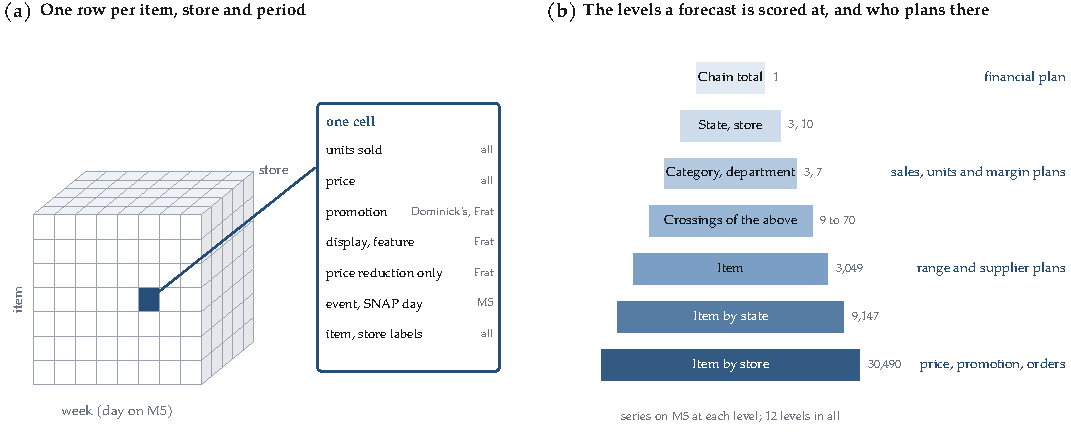
\includegraphics[width=\textwidth]{figs/fig_cube.pdf}
\caption{\textbf{Every data set is one table of item, store and period, scored
at every level a retailer plans at.} \textbf{(a)} Each cell holds the units sold,
the price and whatever plan the data set records; a lever a data set does not
record is passed to the models as unknown, not as zero. \textbf{(b)} The M5
hierarchy with the number of series at each level, and the decisions usually
made at each. Dominick's and Frat have six levels: total, category, store,
category by store, item and item by store; Favorita has total, store, family,
store by family, item and item by store.}
\label{fig:cube}
\end{figure*}

All four data sets are public (Table~\ref{tab:data}) and share one table shape
(Figure~\ref{fig:cube}a). \emph{M5} holds daily Walmart sales of 3,049 items in 10
stores across three states from 2011 to 2016, with prices by week, event days
and the days on which SNAP food assistance is paid~\cite{m5accuracy}.
\emph{Dominick's Finer Foods} holds weekly scanner data by store for a Chicago
chain from 1989 to 1997, with price, a promotion code and cost~\cite{dominicks}.
We use six categories chosen before any final run (cheese, snack crackers, soft
drinks, bottled juice, analgesics, frozen entrees). \emph{Breakfast at the Frat}
holds weekly sales of 55 breakfast items in 77 stores from 2009 to 2012, with
the shelf price, base price, and whether the item was on display, in the weekly
circular (feature) or on a tag-only price reduction~\cite{frat}.
\emph{Corporaci\'on Favorita} holds daily sales of an Ecuadorian grocery chain
to 15 August 2017~\cite{favorita}. It was added in this revision as a data set
kept out of development: the series are the 10 stores with the most units sold
in 2016 crossed with the items sold in all ten that year, from 1 January 2015;
returns are set to zero; the plan is the promotion flag, national holidays and
events, and paydays (the 15th and the last day of each month). Favorita records
no prices, so its WRMSSE weights are unit weights, not revenue weights. No raw
data is redistributed.

\begin{table}[t]
\centering
\caption{\textbf{Four public data sets, all scored item by store and at every
level above it.} Rolling windows were added in this revision and precede every
window used for development.}
\label{tab:data}
\footnotesize
\renewcommand{\arraystretch}{1.2}
\setlength{\tabcolsep}{4pt}
\begin{tabular}{p{0.17\columnwidth}p{0.14\columnwidth}p{0.27\columnwidth}p{0.28\columnwidth}}
\toprule
\textbf{Data} & \textbf{Series} & \textbf{Plan inputs} & \textbf{Rolling windows} \\
\midrule
M5 (daily) & 30,490 & Price, event days, SNAP days & Four of 28 days, Nov 2015 to Feb 2016 \\
Dominick's (weekly) & Six categories & Price, promotion & Six of 8 weeks per category \\
Frat (weekly) & 3,909 & Price, promotion, display, feature, price reduction only & Four of 8 weeks \\
Favorita (daily) & Top 10 stores & Promotion, holidays and events, paydays & Four of 28 days, the last ending 15 Aug 2017 \\
\bottomrule
\end{tabular}
\end{table}

\paragraph{Measure}
We use the weighted root mean squared scaled error (WRMSSE) of
M5~\cite{m5accuracy} at each level of the hierarchy: 12 levels on M5
(Figure~\ref{fig:cube}b) and six on the others. For a level with series $j$,
history $y_{j,1},\dots,y_{j,T}$ before the window and forecasts $\hat y_{j,t}$
for the $H$ periods after it,
\begin{gather}
\mathrm{RMSSE}_j = \sqrt{\frac{\tfrac1H\sum_{t=T+1}^{T+H}(y_{j,t}-\hat y_{j,t})^2}
{\tfrac{1}{T-t_j}\sum_{t=t_j+1}^{T}(y_{j,t}-y_{j,t-1})^2}},\\
\mathrm{WRMSSE} = \textstyle\sum_j w_j\,\mathrm{RMSSE}_j ,
\end{gather}
where $t_j$ is the series' first period with sales and $w_j$ is its share of the
level's dollar sales (units on Favorita) over the last weeks of training. We
report item by store, where orders and promotions are decided, the chain total,
which a financial plan is set against, and the mean over all levels (the M5
score). Each Dominick's data set is one category, so its category level repeats
the total and its category-by-store level repeats the store level; the results
count each distinct level once, four levels on Dominick's. Lower is better.

% =====================================================================
\section{Models}
\label{sec:models}

Table~\ref{tab:models} lists every model. The world model and LightGBM were
each tuned on every data set by the same search (Section~\ref{sec:loop}); their
final settings are in Table~\ref{tab:final-settings}, and the constraints each
works within are in Appendix~\ref{sec:constraints}. Each tuned model's forecast
is the average of five fits with different seeds, except on M5, where each
model is a single fit to bound the cost of the larger data set.

\begin{table}[t]
\centering
\caption{\textbf{Every forecast compared.} Plan: sees the plan for the
forecast periods. Trained: fitted on the data set. Tuned: settings set by the
search of Section~\ref{sec:loop}.}
\label{tab:models}
\footnotesize
\renewcommand{\arraystretch}{1.15}
\setlength{\tabcolsep}{3pt}
\begin{tabular}{p{0.30\columnwidth}cccp{0.33\columnwidth}}
\toprule
\textbf{Model} & \textbf{Plan} & \textbf{Trained} & \textbf{Tuned} & \textbf{Technique} \\
\midrule
Average & yes & yes & yes & Equal-weight mean of the world model and LightGBM \\
Three-model ensemble & yes & yes & yes & Equal-weight mean of the world model, LightGBM and TimesFM with the plan \\
World model & yes & yes & yes & Item state rolled forward under the plan \\
LightGBM & yes & yes & yes & Direct gradient-boosted trees \\
Temporal Fusion Transformer & yes & yes & no & Attention over history and plan \\
TimesFM with the plan & yes & no & no & TimesFM~2.5 with its covariate method \\
Timestral with the plan & yes & no & no & Timestral-28M with known future inputs \\
TimesFM & no & no & no & TimesFM~2.5, 512 periods of units \\
Chronos-Bolt & no & no & no & Chronos-Bolt base \\
Seasonal naive & no & no & no & Sales one season earlier \\
\bottomrule
\end{tabular}
\end{table}

\subsection{World model}

\paragraph{Encoder and state}
For item $i$ in one store, an encoder (a transformer over the last $L$
periods) reads sales and price, each scaled by the item's recent level
$\ell_i$, together with the calendar and the recorded levers, and gives a
state $s_t$; the item and store labels enter the readout. The item's level is
its average over the history window, or, on Dominick's, over its last 8 weeks.

\paragraph{Transition}
A gated recurrent transition $f$ carries the state forward under the plan
$p_{t+h}$ for each future period,
\begin{equation}
s_{t+h}(p) = \mathrm{LN}\big(f(p_{t+h},\, s_{t+h-1}(p))\big), \quad s_t(p) = s_t,
\end{equation}
where LN is layer normalisation (used on M5, Dominick's and Favorita). The plan
holds the period's price as a share of the item's regular price (its highest
price in the last 12 periods) and the recorded levers.

\paragraph{Readout and loss}
Expected sales are a baseline under the ``nothing planned'' plan $p^0$ (regular
price, no lever) times a lift,
\begin{equation}
\begin{split}
\log \mu_{i,t+h} = {} & \log \ell_i + b\big(s_{t+h}(p^0), p^0_{t+h}\big) \\
 & + g\big(s_{t+h}(p), p_{t+h}\big) - g\big(s_{t+h}(p^0), p^0_{t+h}\big),
\end{split}
\end{equation}
with $b$ and $g$ small networks that also take the item's labels and the
horizon step, and the log forecast bounded to $[-10, 10]$. The lift is exactly
zero when nothing is planned, and the baseline does not move when the plan
changes; both are checked by tests in the repository. Training minimises the
loss of Section~\ref{sec:losses} on sales relative to $\ell_i$, with batches of
item, store and date drawn at random.

\paragraph{Brand switching (Dominick's)}
In a store and week where several items are promoted, much of each item's lift
is taken from the others. Following attraction models~\cite{bell1975,cooper1988},
the world model fits on the last 8 training weeks one number per run, the share
$\alpha$ of the summed lift that the category total keeps, and rescales its item
forecasts in each store and week so that the category total is the baseline
total plus $\alpha$ times the summed lift: with baselines $b_i$, lifts
$\lambda_i$ and forecasts $\hat y_i = b_i + \lambda_i$ for the items $i$ of one
store and week,
\begin{equation}
\hat y_i' = \hat y_i\,\frac{\sum_k b_k + \alpha\sum_k \lambda_k}{\sum_k \hat y_k},
\end{equation}
so each item keeps its share of the category forecast. With $\Lambda_g$ the summed
lift and $G_g$ the actual minus baseline sales of store-week group $g$ in the
last 8 training weeks, $\alpha$ is the least-squares slope
$\sum_g \Lambda_g G_g / \sum_g \Lambda_g^2$, kept between 0 and 1.
$\alpha$ is a forecast-implied split
of lift, not an identified estimate of where promoted sales come from, because
promotions are not assigned at random.

\begin{table*}[t]
\centering\footnotesize\setlength{\tabcolsep}{4pt}
\caption{The tuned settings used for every result of Section~\ref{sec:results}, read from the final configurations.
Copies: forecasts averaged over that many fits with different seeds. Size: state width by encoder layers. Steps:
training steps (and pretraining steps on the latent objective, where used). Periods: training periods read. The
changes each search kept are listed in Table~\ref{tab:loop}.}
\label{tab:final-settings}
\begin{tabular}{l ccccc cccc}
\toprule
 & \multicolumn{5}{c}{World model} & \multicolumn{4}{c}{LightGBM}\\
\cmidrule(lr){2-6}\cmidrule(lr){7-10}
Data set & Copies & Size & Steps & Periods & Loss & Copies & Rounds & Periods & Objective\\
\midrule
M5 & 1 & 128$\times$3 & 30,000 & 730 & Hurdle negative binomial & 1 & 800 & 730 & Tweedie \\
Favorita & 5 & 128$\times$3 & 30,000 & 730 & Hurdle negative binomial & 5 & 800 & 730 & Poisson \\
Frat & 5 & 64$\times$2 & 3,000 & 90 & Tweedie & 5 & 500 & 90 & Tweedie \\
Analgesics & 5 & 64$\times$2 & 6,000 & 156 & Tweedie & 5 & 500 & 156 & Tweedie \\
Bottled juice & 5 & 64$\times$2 & 6,000 & 156 & Tweedie & 5 & 500 & 156 & Poisson \\
Cheese & 5 & 64$\times$2 & 6,000 & 156 & Tweedie & 5 & 500 & 156 & Tweedie \\
Frozen entrees & 5 & 64$\times$2 & 6,000 & 156 & Tweedie & 5 & 500 & 156 & Tweedie \\
Soft drinks & 5 & 64$\times$2 & 6,000 & 156 & Tweedie & 5 & 500 & 156 & Tweedie \\
Snacks & 5 & 64$\times$2 & 6,000, pretrained 18,000 steps & 156 & Negative binomial & 5 & 1000 & 156 & Tweedie \\
\bottomrule
\end{tabular}
\end{table*}


\subsection{Training losses}
\label{sec:losses}

\paragraph{The loss used}
The world model is trained on sales relative to the item's level,
$z = y/\ell_i$, by default with the Tweedie deviance for a mean $\mu$ and power
$p = 1.5$,
\begin{equation}
L_p(z, \mu) = -\frac{z\,\mu^{1-p}}{1-p} + \frac{\mu^{2-p}}{2-p},
\end{equation}
the negative log-likelihood, up to terms free of $\mu$, of a compound
Poisson--gamma distribution with a point mass at zero~\cite{jorgensen1987}.
Because the loss is on $z$, every item counts alike whatever its volume. The
search replaced it on three data sets (Table~\ref{tab:final-settings}): on M5
and Favorita by a hurdle negative binomial, a probability of any sale times a
negative binomial for the units sold when there is one, and on snacks by a
negative binomial; in each the spread of the negative binomial is learnt for
each item. LightGBM uses the Tweedie deviance with $p = 1.1$ on units, so large
items count for more, or the Poisson deviance where its search chose it, and the
Temporal Fusion Transformer a negative binomial likelihood on units.

\paragraph{The changes tried}
Each change below adds to or replaces $L_p$ for one batch $B$ of item, store and
period examples. Table~\ref{tab:losses} scores each against the configuration it
changed in the first revision, where none was kept; the search of
Section~\ref{sec:loop} tried them again on the tuned settings, with the
likelihoods above, and kept the changes listed in Table~\ref{tab:loop}.
\begin{itemize}\setlength{\itemsep}{1pt}
\item \emph{Negative binomial} on units, $-\log\mathrm{NB}(y;\,\mu\ell_i, r)$
with the spread $r$ learnt.
\item \emph{Totals term}: the loss adds
$\lambda_T\,\mathrm{mean}_t\big[(\sum_{b\in B_t}\hat y_b - \sum_{b\in B_t} y_b) /
\max(1, \sum_{b\in B_t} y_b)\big]^2$, the relative gap between summed forecasts
and sales over the examples $B_t$ sharing a date, so that a small bias in the
same direction on many items is penalised ($\lambda_T = 1$).
\item \emph{Volume and dollar weights}: each example's loss times
$\ell_i^{\,\gamma}$, or $(\ell_i\bar\pi_i)^{\gamma}$ with $\bar\pi_i$ the item's
usual price, normalised to mean one in the batch, with $\gamma = 0.9$ and
$p = 1.1$, which makes the loss close to LightGBM's on units or dollars.
\item \emph{Peak weight}: each period's loss times
$1 + \kappa\min(|z_t - 1|, 5)$, normalised to mean one, so that peaks and dips
count for more ($\kappa = 0.5$, with the dollar weight above).
\item \emph{After-promotion weight}: each period with no lever on that follows a
period with one counts $1 + w$ times, normalised to mean one ($w = 2$ or $5$).
\item \emph{Latent term}: from the state now and the plan, the transition
predicts the state the encoder gives once those periods are history, against a
slowly updated copy of the encoder; the loss adds
$\lambda_Z \sum_h \delta^h \lVert s_{t+h}(p) - \bar s_{t+h}\rVert^2$ with
$\delta \le 1$ discounting far periods, and optionally a variance and covariance
penalty on the state~\cite{vicreg}. It was also used alone to pretrain the
encoder, which was then frozen, trained at a lower rate or trained fully on the
forecast loss.
\end{itemize}

\begin{table*}[t]
\centering
\caption{\textbf{No change to the training loss became a default: each was lower in error than the configuration
it changed in at most half its comparisons.} Each row is one change to the Tweedie loss of the world model or lift
model, scored on the development windows against the configuration with the same data, windows and every other
setting. WRMSSE: overall (mean of the hierarchy levels), averaged over the seeds and windows both ran and over the
data sets in the row. Lower: the number of data sets (or category and model pairs) in which the change had the lower
error. The weight after a promotion comes from a separate rerun of the world model in the same job. Rows marked
not run were configured but have no full-data run in the records. Built by \texttt{scripts/loss\_ledger.py}.}
\label{tab:losses}
\footnotesize
\begin{tabular}{p{0.36\textwidth}p{0.17\textwidth}rrl}
\toprule
\textbf{Change to the loss} & \textbf{Tested on} & \textbf{With it} & \textbf{Without} & \textbf{Result} \\
\midrule
Negative binomial likelihood & Dominick's, Frat & 0.537 & 0.541 & Lower in 1 of 2 \\
Totals term & Dominick's, Frat & 0.655 & 0.583 & Lower in 0 of 3 \\
Unit-volume weight and Tweedie power 1.1 & Dominick's & -- & -- & Not run on full data \\
Dollar-volume weight and Tweedie power 1.1 & Dominick's & -- & -- & Not run on full data \\
Peak weight, dollar weight and Tweedie power 1.1 & Dominick's & 0.853 & 0.856 & Lower in 5 of 12 \\
Weight 3 on the periods after a promotion & Dominick's & 0.834 & 0.832 & Lower in 2 of 6 \\
Weight 6 on the periods after a promotion & Dominick's & 0.810 & 0.832 & Lower in 2 of 6 \\
Latent term, weight 0.1 & Frat & 0.411 & 0.406 & Lower in 0 of 1 \\
Latent term, weight 0.5 & Frat & 0.414 & 0.407 & Lower in 0 of 2 \\
Latent term, weight 2 & Frat & 0.410 & 0.406 & Lower in 0 of 1 \\
Latent term with a spread penalty and discount & Dominick's, Frat & 0.567 & 0.549 & Lower in 0 of 4 \\
Latent pretraining, encoder frozen afterwards & Frat & 0.428 & 0.406 & Lower in 0 of 1 \\
Latent pretraining, encoder full afterwards & Frat & 0.407 & 0.406 & Lower in 0 of 1 \\
Latent pretraining, encoder at a lower rate afterwards & Frat & 0.411 & 0.407 & Lower in 0 of 3 \\
Latent pretraining, then forecast with the latent term & Frat & 0.415 & 0.406 & Lower in 0 of 1 \\
Latent pretraining, then forecast with a totals term & Dominick's, Frat & 0.729 & 0.667 & Lower in 0 of 1 \\
\bottomrule
\end{tabular}
\end{table*}


\subsection{Average and ensemble}
The average is the equal-weight mean of the tuned world model's and the tuned
LightGBM's forecasts for each item, store and period, with no weights fitted.
The three-model ensemble adds TimesFM with the plan, also with equal weights; it
was fixed on 13 October 2026, before any result of the revision, and is reported
beside the average. The forecast by history of Section~\ref{sec:rq-broad} uses
the world model alone for series with less than 26 weeks of sales and the
average for the rest.

\subsection{Comparison models}
\emph{LightGBM}~\cite{lightgbm}: a direct model, one per store on M5 and
Favorita, reading sales at lags no shorter than the horizon, rolling averages and
spread of sales, price against the item's highest recent price, the calendar and
the plan inputs, with the item as a label; tuned as in Table~\ref{tab:final-settings}.
\emph{Temporal Fusion Transformer}~\cite{tft}: one model per data set on
Dominick's and Frat, fitted on the last 156 weeks with the plan as known future
inputs and a negative binomial likelihood, 1,500 steps; it was not run on M5, where its
training cost was beyond the compute available, nor on Favorita, whose model
list was fixed without it. Chronos-Bolt and TimesFM from history alone were
not run on Favorita either. \emph{TimesFM}~\cite{timesfm,timesfm25}:
the 200M-parameter TimesFM~2.5 checkpoint given each series' last 512 periods;
we use its mean output, chosen in the first version because its median forecast
fell well below M5 totals, as the median of intermittent daily sales does. \emph{TimesFM with the plan}: the same model
through its covariate method, a linear model on the plan inputs fitted over
groups of 2,048 series, then TimesFM on what that model leaves.
\emph{Chronos-Bolt}~\cite{chronos}: the base checkpoint, zero-shot, the mean of
its quantiles. \emph{Timestral}~\cite{timestral}: Timestral-28M (code commit
a534bdb), zero-shot, with the plan as known future inputs (price relative to
the context's highest price, other levers as given) and from history alone;
the point forecast is the mean of its 21 quantiles, each weighted by the share
of probability nearest it. \emph{Seasonal naive}: sales one season earlier.

% =====================================================================
\section{Experimental setup}
\label{sec:setup}

\paragraph{Windows}
Every result of Section~\ref{sec:results} is scored on rolling windows that no
choice of setting ever saw: six 8-week windows on each Dominick's category, four
on Frat, and four 28-day windows on M5 (November 2015 to February 2016) and on
Favorita (the last ending on its last day), each forecast from everything
earlier. The searches of Section~\ref{sec:loop} scored windows before these,
and held the latest of their own windows out of every decision. The windows used
to develop the first version of the models lie after the rolling windows and are
not scored in this paper (Figure~\ref{fig:study}a).

\paragraph{Rules fixed in advance}
The revision plan, with every window, model, test and pass rule, was written down
before the revision's first run, and every change to it is a dated entry,
made before the results it governs were read unless the entry says otherwise.
Each data set's world model and LightGBM run in every rolling window with the
final settings of their searches (Table~\ref{tab:final-settings}), unchanged
from window to window; each forecast is the average of five fits with different
seeds (a single fit on M5). No result on the rolling windows changed a
setting, and every model, window and test is reported.

\paragraph{Comparing two models}
For models $A$ and $B$, window $k$ and a level, let $d_k = \mathrm{WRMSSE}_k(A) -
\mathrm{WRMSSE}_k(B)$. Within a window, $d_k$ gets a 95\% interval from 1,000
resamples of items: an item drawn twice counts twice in every series and
aggregate it feeds, with the weights recomputed. Across the $K$ windows, the
mean $\bar d = \frac1K\sum_k d_k$ gets a 95\% interval from the 2.5\% and 97.5\%
quantiles of $\bar d^{*}$ over 5,000 resamples of windows with replacement. A
model is said to beat another only when that interval excludes zero;
when it does not, we say no difference was detected, which is not a finding that
the two are equal. For each data set and level we report the 90\% model
confidence set~\cite{hansen2011}: starting from all models $\mathcal M$, the range
statistic $T = \max_{a,b\in\mathcal M} |\bar d_{ab}|/\hat\sigma_{ab}$, with
$\hat\sigma_{ab}$ from the bootstrap over windows, is compared with its
bootstrap distribution under equal expected loss (5,000 resamples); while the
$p$-value is below 0.10 the model whose standardised losses against the others
are largest is removed, and the models left form the set. With four to six windows these tests have little power, and adjacent
windows are dependent: each is forecast from all data before it, so they share
most of their training history, and an error tied to a season or a stretch of
trading can recur in neighbouring windows. A bootstrap that resamples whole
windows treats them as exchangeable and so understates that dependence; we
therefore also count, over levels and windows, the comparisons in which one model
is clearly more accurate than the other by the item bootstrap
(Section~\ref{sec:rq-grain}).

\paragraph{Intervals}
Each model's interval forecasts come from its own errors in the earlier rolling
windows of the same data set, a rolling form of conformal
calibration~\cite{vovk2005}. With $e_{j,h} = (y_{j,t+h} - \hat y_{j,t+h})/\sigma_j$
the scaled errors of the earlier windows at horizon $h$ ($\sigma_j$ the series'
one-step scale), the interval at level $1-\alpha$ is
$\big[\hat y_{j,t+h} + \sigma_j q_{\alpha/2,h},\ \hat y_{j,t+h} + \sigma_j
q_{1-\alpha/2,h}\big]$, with $q_{\cdot,h}$ the empirical quantiles of the pooled
$e_{\cdot,h}$. Where a level has fewer than 50
earlier errors for each horizon, all horizons are pooled into one set of
quantiles, and interval ends are rounded outwards to whole units except on
Favorita; this fix was added on 16 October after the first intervals covered
far less than planned at the totals, and is used throughout. The first
rolling window has no earlier window and is not scored. We report the scaled
pinball loss averaged over the quantiles, weighted as in the M5 uncertainty
competition~\cite{m5uncertainty}, and coverage at 50\%, 80\% and 95\%. Models
that give quantiles of their own (Chronos-Bolt, TFT) are also scored on them,
over every window.

\paragraph{Decisions}
Three simulations turn forecasts into costs. \emph{Store orders}: for each
item-store-period, order the model's interval quantile at a critical ratio $r$
of 0.5, 0.8 or 0.95; each unit over costs 1 and each unit short $r/(1-r)$.
\emph{Category plan}: for category-by-store nodes $n$ with sales $y_{n,t}$,
forecast $\hat y_{n,t}$ and average price $\bar\pi_n$ before the window,
\begin{equation}
C = \frac{\sum_n \bar\pi_n \sum_{t} |y_{n,t} - \hat y_{n,t}|}{\sum_n \bar\pi_n \sum_t y_{n,t}},
\end{equation}
the absolute error in dollars over sales in dollars. \emph{Promotion decisions}: in the generated
store worlds of the companion paper~\cite{paper2}, where each promotion's true
lift is known, promote when the predicted lift times margin exceeds a fixed
cost; regret is the value lost against deciding with the true lift. The first
two are reported against seasonal naive. All are simulations under stated
costs, not business results.

\paragraph{Reconciliation}
Base forecasts at every node come from AutoETS fitted on the history before each
window (seasonal at the aggregate nodes, non-seasonal item by store). They are
reconciled bottom-up, top-down by historical proportions, and by the MinT
family~\cite{mint}. With $S$ the summing matrix (nodes by item-store series) and
$\hat{\mathbf y}$ the base forecasts at every node, the reconciled item-store
forecasts are
\begin{equation}
\tilde{\mathbf b} = (S^\top W^{-1} S)^{-1} S^\top W^{-1}\hat{\mathbf y},
\end{equation}
with $W = I$ (ordinary least squares), $W = \mathrm{diag}(S\mathbf 1)$ (structural
weights), $W$ the diagonal of in-sample error variances, or $W = \lambda
\mathrm{diag}(\hat\Sigma) + (1-\lambda)\hat\Sigma$ with the Sch\"afer--Strimmer
intensity $\lambda$ (MinT-shrink, where the hierarchy has at most 6,000 nodes:
Frat); nodes with no
in-sample error are given the smallest variance of the others. Each model's own
item-by-store forecasts are also combined with ETS above them by weighted least
squares.

\paragraph{Ranking}
Accuracy says how close a forecast is, not whether it puts items in the right
order. For every window we report the Spearman correlation, across item-store
series that sold in the window before, between the forecast change (horizon
total over the previous horizon's total) and the actual change; the share of the
tenth of nodes forecast to grow most that are in the actual top tenth (0.10 by
chance); the Spearman correlation across promoted periods between forecast and
actual units over the series' unpromoted level; and bias, forecast over actual.
These were written down before they ran and have no pass rule.

\paragraph{Analyses added after the first results}
Four analyses were added after the first scores of the tuned models were read,
each written down before it ran: the scores by line type (Section~\ref{sec:rq-lines});
the whole window scored as one block; the average and the forecast by history on
the transfer test's kept-out series (Section~\ref{sec:rq-unseen}); and the
supporting analyses of Section~\ref{sec:support} rerun on the tuned models. The
transfer test and the pooled training of RQ4 were written down before any
tuned model was scored.

% The research loop: how both models' settings were searched (revision, November 2026).
% Numbers come from paper/generated/tab_loop.tex and the figures, all built from results/research/*/log.jsonl
% by paper/figs/make_loop_figures.py.
\section{Searching the settings of both models}
\label{sec:loop}

Both models were tuned with the same procedure on every data set. On the windows the searches
scored, tuning improved LightGBM on all \loopImprovedLgb{} data sets and the world model on \loopImprovedWm{}, and the gains
were mostly small next to the differences between data sets. The held-out window agreed with the
search windows only weakly, so the paper judges the models on later windows the searches never
saw. Table~\ref{tab:loop} gives every search from its starting settings to its final settings, and
Figure~\ref{fig:looppath} shows every run in the order it was made.

\subsection{The procedure}

The procedure is a fixed loop, written down before it ran, that changes one setting at a time. It
starts from the settings the first version of this paper used. Each change on a menu fixed in
advance is run once, on one seed, on top of the best settings so far. Every change that beats the
best settings on that seed is run on two more seeds. The best of those is kept if its mean over
three seeds beats the best settings' mean by at least the keep bar, which is the spread of the
three seeds of the starting settings. The loop then starts a new round from the new best and stops
when a round keeps nothing. A change cannot be kept because one seed was lucky, and the bar is set
by the model's own noise on that data set before any change is tried.

The windows the loop scores lie before every window this paper reports. The latest of them is held
out: it is scored for every three-seed run and never used to decide. The menus differ between the
models, because the models have different settings, but each covers what a practitioner would try
first: for the world model the loss weights, the roll-forward, training length, learning rate and
batch, weight averaging and the latent checks of Section~\ref{sec:models}; for LightGBM the
number of leaves, the learning rate and number of rounds, the minimum data in a leaf, the
objective, feature sampling and the lag windows.

After its loop each world model had two more rounds of one change each. The first tried four count
likelihoods that treat weeks with no sales on their own: the negative binomial, the same with a
spread for each item, the zero-inflated negative binomial and the hurdle negative binomial. The
second tried JEPA pretraining of the encoder with the forecast head fitted afterwards at a lower
rate, at two lengths of pretraining. Both used the keep rule above. LightGBM has no counterpart
to either, so it had none. Pretraining used only each data set's own history, so the two models
still saw the same data.

Each model on each data set was searched as a five-copy average, the mean forecast of five fits
with different seeds, except on M5, where both models were single fits. Section~\ref{sec:loopnoise} shows why the
average matters.

\begin{table*}[t]
\centering\footnotesize
\caption{Every search, from starting to final settings. Scores are WRMSSE (lower is better), the mean of three seeds on the search windows and one score on the held-out window, which never decided anything. The keep bar is the seed spread of the starting settings; a change was kept only when its three-seed mean beat the best so far by at least the bar. Tries counts every run, first-seed screens and three-seed confirmations.}
\label{tab:loop}
\begin{tabular}{llrrrrrrp{5.2cm}}
\toprule
Data & Model & Tries & Keep bar & \multicolumn{2}{c}{Starting} & \multicolumn{2}{c}{Final} & Kept, in order \\
& & & & Search & Held-out & Search & Held-out & \\
\midrule
M5 & World model & 59 & 0.013 & 0.570 & 0.550 & 0.533 & 0.534 & feedback, hurdle nb item spread \\
 & LightGBM & 51 & 0.003 & 0.603 & 0.553 & 0.556 & 0.522 & num leaves quarter \\
\addlinespace[2pt]
Favorita & World model & 51 & 0.028 & 0.547 & 0.600 & 0.483 & 0.560 & latent overshooting \\
 & LightGBM & 99 & 0.009 & 0.922 & 0.576 & 0.580 & 0.573 & min data in leaf 4x, objective poisson, learning rate half \\
\addlinespace[2pt]
Frat & World model & 53 & 0.028 & 0.588 & 0.591 & 0.547 & 0.608 & batch half \\
 & LightGBM & 52 & 0.003 & 0.501 & 0.546 & 0.489 & 0.546 & learning rate double \\
\addlinespace[2pt]
Analgesics & World model & 35 & 0.004 & 0.509 & 0.619 & 0.509 & 0.619 & nothing \\
 & LightGBM & 52 & 0.010 & 0.548 & 0.757 & 0.528 & 0.764 & num leaves quarter \\
\addlinespace[2pt]
Bottled juice & World model & 30 & 0.028 & 0.587 & 0.637 & 0.587 & 0.637 & nothing \\
 & LightGBM & 67 & 0.008 & 0.708 & 0.582 & 0.674 & 0.593 & objective poisson, feature fraction 0.8 \\
\addlinespace[2pt]
Cheese & World model & 33 & 0.034 & 0.392 & 0.714 & 0.392 & 0.714 & nothing \\
 & LightGBM & 49 & 0.002 & 0.352 & 0.833 & 0.346 & 0.839 & longer windows \\
\addlinespace[2pt]
Frozen entrees & World model & 95 & 0.007 & 0.246 & 0.251 & 0.216 & 0.241 & total weight 0.1, batch half \\
 & LightGBM & 53 & 0.010 & 0.222 & 0.183 & 0.181 & 0.195 & num leaves 4x \\
\addlinespace[2pt]
Soft drinks & World model & 65 & 0.020 & 0.594 & 0.579 & 0.572 & 0.522 & lr double \\
 & LightGBM & 80 & 0.004 & 0.554 & 0.435 & 0.532 & 0.507 & num leaves quarter, max bin 255 \\
\addlinespace[2pt]
Snacks & World model & 42 & 0.018 & 0.439 & 0.568 & 0.400 & 0.608 & negative binomial item spread, jepa hybrid long \\
 & LightGBM & 54 & 0.006 & 0.358 & 0.425 & 0.351 & 0.424 & rounds double \\
\addlinespace[2pt]
\bottomrule
\end{tabular}
\end{table*}


\begin{figure*}[t]
\centering
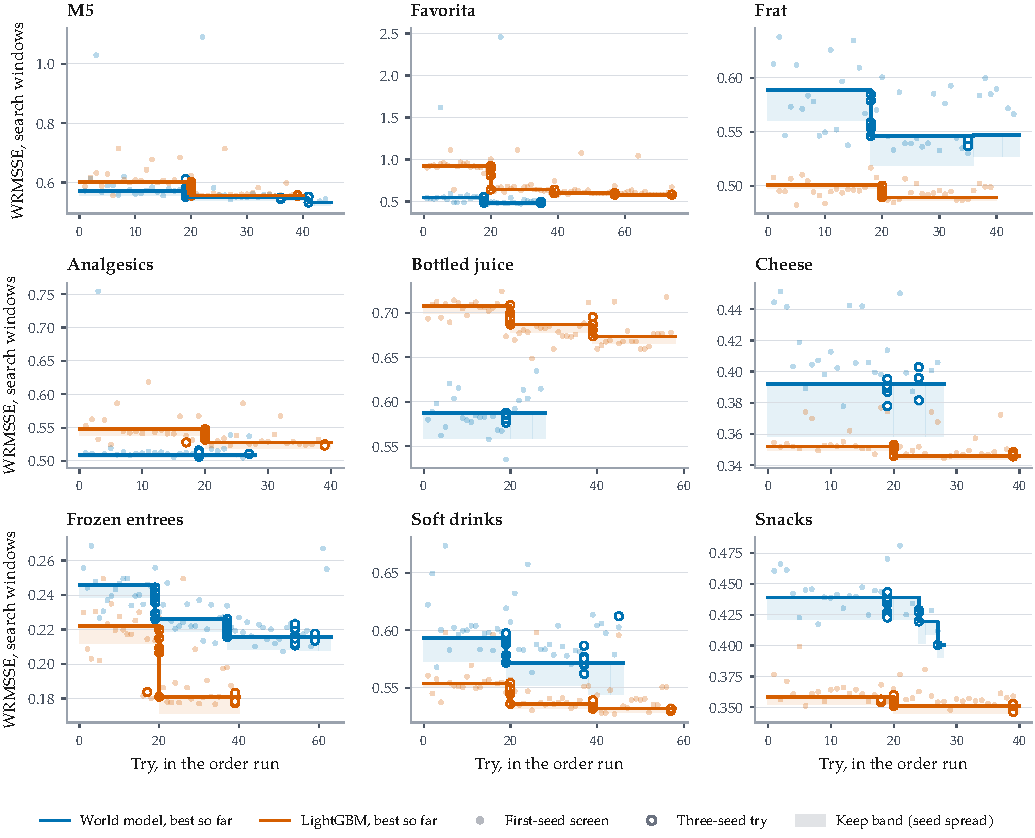
\includegraphics[width=\textwidth]{figs/fig_loop_path.pdf}
\caption{Every run of every search, in the order it was made. Faint dots are first-seed screens,
open circles are three-seed confirmations, and the step line is the best settings so far. The band
under the line is the keep bar: a change had to land below it to be kept. The world model's line
runs on into its likelihood and JEPA rounds after its own loop ends.}
\label{fig:looppath}
\end{figure*}

\subsection{What the searches kept}

The searches made \loopTries{} runs, \loopTriesWm{} of the world model and \loopTriesLgb{} of LightGBM, and kept \loopKept{} changes, \loopKeptWm{} for the world model and \loopKeptLgb{} for LightGBM.
LightGBM kept at least one change on every data set and the world model kept nothing on three of
the six Dominick's categories. No single change helped the world model everywhere
(Figure~\ref{fig:loopheat}). Weighting the loss toward high-volume series made the first seed worse on most data sets. The seven-step latent
check, kept on Favorita, was among the changes that moved Favorita most and did little elsewhere.

On the search windows the world model improved on \loopImprovedWm{} of the nine data sets and LightGBM on all
\loopImprovedLgb{} (Figure~\ref{fig:loopslopes}). The largest gain of either model was LightGBM on \loopGainLgbSet{},
from \loopGainLgbFrom{} to \loopGainLgbTo{}. The world model's largest was on \loopGainWmSet{}, from \loopGainWmFrom{} to \loopGainWmTo{}.

\begin{figure}[t]
\centering
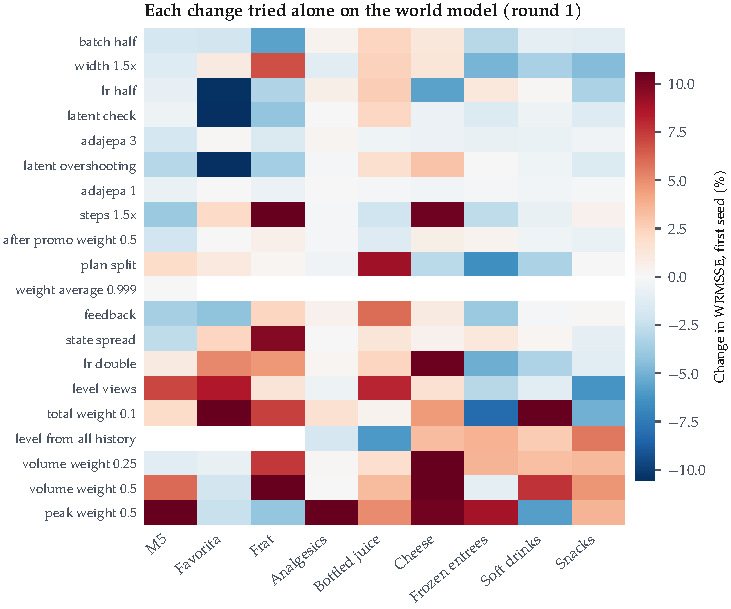
\includegraphics[width=\columnwidth]{figs/fig_loop_heat.pdf}
\caption{Each change tried alone on the world model in the first round, against that data set's
starting settings on the first seed. Blue is better. A blank cell is a change that was not on that
data set's menu.}
\label{fig:loopheat}
\end{figure}

\subsection{Did the held-out window agree?}

Only partly. Across every three-seed run, the change on the search windows and the change on the
held-out window are correlated at \loopHeldCorrWm{} for the world model and \loopHeldCorrLgb{} for LightGBM
(Figure~\ref{fig:loopheldout}). A change that helps on the search windows is a weak guide to the
next window. The world model's final settings were worse than its starting settings on the
held-out window on \loopHeldWorseWm{} data sets, most on \loopHeldWorstWmSet{} (\loopHeldWorstWmFrom{} to \loopHeldWorstWmTo{}), and
LightGBM's on \loopHeldWorseLgb{}, most on \loopHeldWorstLgbSet{} (\loopHeldWorstLgbFrom{} to \loopHeldWorstLgbTo{}). This is why the paper reports the final settings on windows that the
searches never saw, in Section~\ref{sec:results}, and not the search scores.

\begin{figure}[t]
\centering
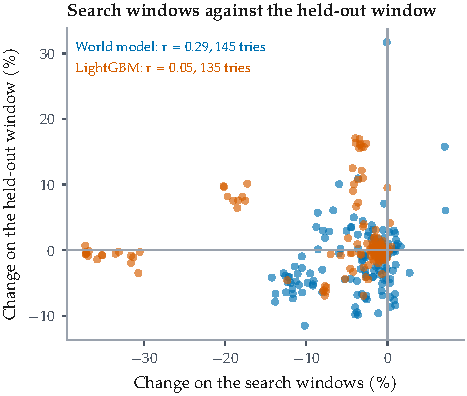
\includegraphics[width=\columnwidth]{figs/fig_loop_heldout.pdf}
\caption{Each three-seed run's change on the search windows against its change on the held-out
window, both against the starting settings of its search.}
\label{fig:loopheldout}
\end{figure}

\subsection{Seed noise, one copy against five}
\label{sec:loopnoise}

A single world-model fit is noisy enough to hide most of the changes the loop tries. On the six
Dominick's categories the three seeds of the starting settings differ from their mean by a
standard deviation of \loopSeedSdOne\% for a single fit and \loopSeedSdFive\% for a five-copy average
(Figure~\ref{fig:loopnoise}). The
single-fit search on cheese had a bar of \loopOneCheBar{} and kept nothing; with the average the bars on the
Dominick's categories were between \loopBarLoWm{} and \loopBarHiWm{}. LightGBM's seeds differ much less, and its
bars were between \loopBarLoLgb{} and \loopBarHiLgb{}.

\begin{figure}[t]
\centering
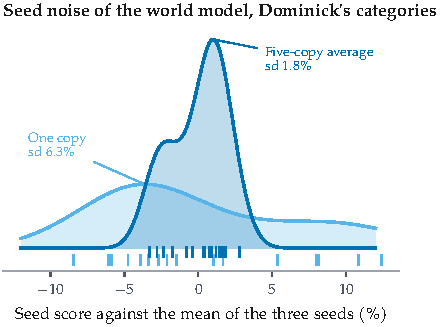
\includegraphics[width=\columnwidth]{figs/fig_loop_noise.pdf}
\caption{The starting settings' three seed scores on each Dominick's category, as a share of their
mean, for a single world-model fit and for the five-copy average. Ticks are the scores.}
\label{fig:loopnoise}
\end{figure}

\begin{figure*}[t]
\centering
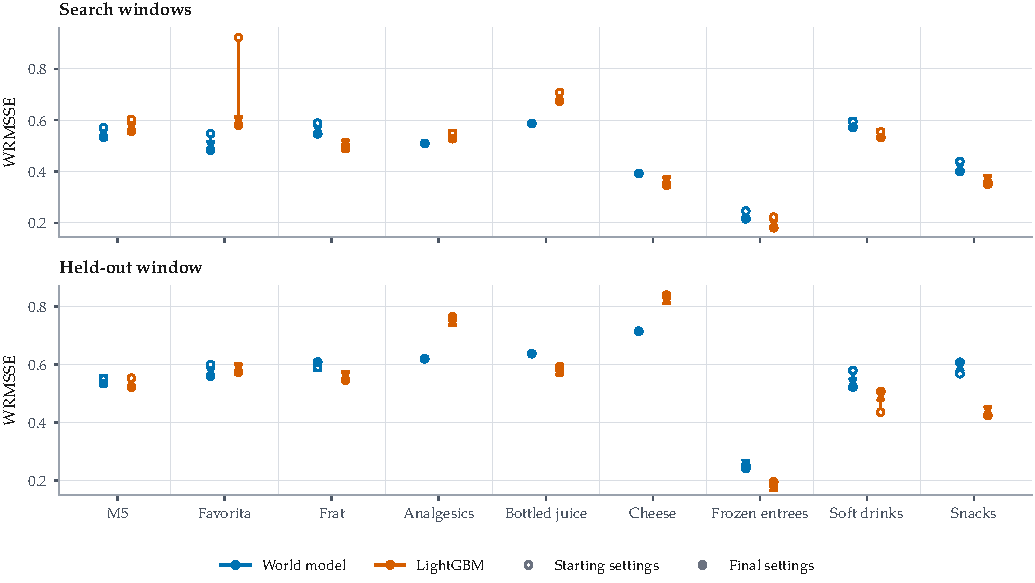
\includegraphics[width=\textwidth]{figs/fig_loop_slopes.pdf}
\caption{Each model's starting and final settings on each data set. Open circles are the starting
settings and filled circles the final settings, on the search windows (top) and the held-out
window (bottom).}
\label{fig:loopslopes}
\end{figure*}

% =====================================================================
\section{Results}
\label{sec:results}

% Results by research question (Framework section). Tables from scripts/make_rq_tables.py; paired counts from
% results/analysis_tuned/paired.csv (item bootstrap within each window, 90% intervals).
\newcommand{\rqAvgBestCoarse}{8}
\newcommand{\rqAvgBestItem}{9}
\newcommand{\rqAvgBestBlock}{5}
\newcommand{\rqAvgBestCoarseWord}{eight}
\newcommand{\rqAvgBestItemWord}{nine}
\newcommand{\rqAvgBestBlockWord}{five}
\newcommand{\rqCells}{27}
\newcommand{\rqAvgBestCells}{22}
\newcommand{\rqAvgWorstCells}{0}
\newcommand{\rqWmWorstCells}{16}
\newcommand{\rqLgbWorstCells}{11}
\newcommand{\rqAvgSecondBlock}{4}
\newcommand{\rqBlockMfiveWm}{0.598}
\newcommand{\rqBlockMfiveLgb}{0.953}
\newcommand{\rqBlockMfiveAvg}{0.589}
\newcommand{\rqBlockFavWm}{0.482}
\newcommand{\rqBlockFavLgb}{0.565}
\newcommand{\rqBlockFavAvg}{0.412}
\newcommand{\rqBlockSdrWm}{0.576}
\newcommand{\rqBlockSdrLgb}{0.632}
\newcommand{\rqBlockSdrAvg}{0.470}
\newcommand{\rqPAvgWmBetter}{128}
\newcommand{\rqPAvgWmWorse}{27}
\newcommand{\rqPAvgWmN}{312}
\newcommand{\rqPAvgWmCoarsebetter}{68}
\newcommand{\rqPAvgWmCoarseworse}{19}
\newcommand{\rqPAvgWmCoarsen}{212}
\newcommand{\rqPAvgWmItembetter}{60}
\newcommand{\rqPAvgWmItemworse}{8}
\newcommand{\rqPAvgWmItemn}{100}
\newcommand{\rqPAvgLgbBetter}{124}
\newcommand{\rqPAvgLgbWorse}{21}
\newcommand{\rqPAvgLgbN}{312}
\newcommand{\rqPAvgLgbCoarsebetter}{77}
\newcommand{\rqPAvgLgbCoarseworse}{17}
\newcommand{\rqPAvgLgbCoarsen}{212}
\newcommand{\rqPAvgLgbItembetter}{47}
\newcommand{\rqPAvgLgbItemworse}{4}
\newcommand{\rqPAvgLgbItemn}{100}
\newcommand{\rqPWmLgbBetter}{64}
\newcommand{\rqPWmLgbWorse}{75}
\newcommand{\rqPWmLgbN}{312}
\newcommand{\rqPWmLgbCoarsebetter}{40}
\newcommand{\rqPWmLgbCoarseworse}{45}
\newcommand{\rqPWmLgbCoarsen}{212}
\newcommand{\rqPWmLgbItembetter}{24}
\newcommand{\rqPWmLgbItemworse}{30}
\newcommand{\rqPWmLgbItemn}{100}
\newcommand{\rqAvgItemWorseMax}{8}
\newcommand{\rqMcsWorldModel}{35}
\newcommand{\rqMcsLightgbm}{37}
\newcommand{\rqMcsAverage}{51}
\newcommand{\rqMcsEnsemble}{41}
\newcommand{\rqMcsTimesfm}{12}
\newcommand{\rqMcsCells}{60}
\newcommand{\rqFastShareDomLo}{11}
\newcommand{\rqFastShareDomHi}{21}
\newcommand{\rqFastShareRestLo}{37}
\newcommand{\rqFastShareRestHi}{42}
\newcommand{\rqShortShareDomLo}{11}
\newcommand{\rqShortShareDomHi}{21}
\newcommand{\rqShortShareRestMax}{2}
\newcommand{\rqAvgBestFast}{eight}
\newcommand{\rqAvgBestSlow}{eight}
\newcommand{\rqShortWmBeatsLgb}{eight}
\newcommand{\rqShortFavWm}{0.539}
\newcommand{\rqShortFavLgb}{0.667}
\newcommand{\rqShortMfiveWm}{0.866}
\newcommand{\rqShortMfiveLgb}{1.024}
\newcommand{\rqNineWord}{nine}
\newcommand{\rqSnaWm}{1.009}
\newcommand{\rqSnaLgb}{0.865}
\newcommand{\rqSnaAvg}{0.884}
\newcommand{\rqRuleLevel}{eight}
\newcommand{\rqRuleSna}{0.970}
\newcommand{\rqCostWmItemLo}{0.008}
\newcommand{\rqCostWmItemHi}{0.040}
\newcommand{\rqCostLgbItemLo}{0.058}
\newcommand{\rqCostLgbItemHi}{0.311}
\newcommand{\rqFaWmItemLo}{89}
\newcommand{\rqFaWmItemHi}{104}
\newcommand{\rqFaLgbItemLo}{66}
\newcommand{\rqFaLgbItemHi}{93}
\newcommand{\rqFaAvgItemLo}{78}
\newcommand{\rqFaAvgItemHi}{96}
\newcommand{\rqWmFaItemOff}{11}
\newcommand{\rqKeptSets}{five}
\newcommand{\rqItemWmBeatsAvg}{five}
\newcommand{\rqStoreWmBeatsLgb}{four}
\newcommand{\rqStoreAvgBeatsWm}{one}
\newcommand{\rqStoreWmBeatsAvg}{one}
\newcommand{\rqStoreLevel}{three}
\newcommand{\rqLgbFaItemLoFrac}{two thirds}
\newcommand{\rqCarriedWm}{0.447}
\newcommand{\rqOwnWm}{0.428}
\newcommand{\rqCarriedLgb}{0.450}
\newcommand{\rqOwnLgb}{0.448}
\newcommand{\rqCarriedWmIxs}{0.002}
\newcommand{\rqCarriedLgbIxs}{0.001}
\newcommand{\rqPoolGainMax}{0.007}
\newcommand{\rqPoolGainWm}{0.005}
\newcommand{\rqPoolGainWmSet}{analgesics}
\newcommand{\rqPoolGainLgb}{0.007}
\newcommand{\rqPoolGainLgbSet}{frozen entrees}
\newcommand{\rqPoolLossWm}{0.141}
\newcommand{\rqPoolLossWmSet}{soft drinks}
\newcommand{\rqPoolLossLgb}{0.235}
\newcommand{\rqPoolLossLgbSet}{analgesics}
\newcommand{\rqPoolGainMaxTwo}{0.01}


The results follow the four research questions. Every number comes from the
tuned world model and the tuned LightGBM, each set by the same search on each
data set (Section~\ref{sec:loop}), scored on the paper's windows. The average is
the equal-weight mean of the two forecasts.

\subsection{RQ1: grain}
\label{sec:rq-grain}

\textbf{Use the average at every grain.} Across the nine data sets and the
three views of Table~\ref{tab:rq-grain} (store grain and above by period, item
grain by period, and the whole window as one block), the average has the lowest
error in 22 of 27 cases and is never the least accurate of the three. The world
model is the least accurate in 16 cases and LightGBM in 11.

The paired tests give the same answer. They compare two forecasts level by level
and window by window, and count a difference only when it holds after
resampling items. Against the world model, the average is clearly more accurate
in 128 of 312 comparisons and clearly less accurate in 27; against LightGBM, 124
and 21. At item grain it is clearly less accurate than either model in at most 8
of 100 comparisons. Across data sets and levels it is in the 90\% model
confidence set in \rqMcsAverage{} of \rqMcsCells{} cases, against
\rqMcsLightgbm{} for LightGBM and \rqMcsWorldModel{} for the world model.

\textbf{Grain does not decide between the two models on their own.} The world
model is clearly more accurate than LightGBM in 40 comparisons at store grain
and above and clearly less accurate in 45; at item grain the counts are 24 and
30. Neither is ahead at either grain across the data sets, so a retailer that
picks one model for a grain is picking by data set, not by grain. The average
removes that choice.

\textbf{On the whole promotion block, the average is again the safe choice.} It
is lowest on five of nine data sets and second on the other four. LightGBM is
lowest on analgesics, bottled juice and snacks, but drifts in total where the
world model does not: its block error on M5 is 0.953, against 0.598 for the world
model and 0.589 for the average, and the same pattern shows on Favorita and soft
drinks.

\begin{table*}[t]
\centering\footnotesize\setlength{\tabcolsep}{3pt}
\caption{RQ1, grain. WRMSSE of the tuned world model (WM), the tuned LightGBM (LGB) and their equal-weight average
(Avg), averaged over the levels at store grain and above, over the item levels, and over every level for the whole
forecast window summed as one block; mean over the paper's windows. Lowest of the three in bold.}
\label{tab:rq-grain}
\resizebox{\textwidth}{!}{\begin{tabular}{l ccc ccc ccc}
\toprule
 & \multicolumn{3}{c}{Store and above, by period} & \multicolumn{3}{c}{Item levels, by period} & \multicolumn{3}{c}{Whole block, all levels}\\
\cmidrule(lr){2-4}\cmidrule(lr){5-7}\cmidrule(lr){8-10}
Data set & WM & LGB & Avg & WM & LGB & Avg & WM & LGB & Avg\\
\midrule
Analgesics & 0.688 & 0.698 & \textbf{0.678} & 0.710 & 0.705 & \textbf{0.695} & 0.523 & \textbf{0.458} & 0.472 \\
Bottled juice & 0.569 & 0.566 & \textbf{0.539} & 0.581 & 0.596 & \textbf{0.563} & 0.545 & \textbf{0.404} & 0.445 \\
Cheese & 0.381 & 0.471 & \textbf{0.377} & 0.623 & 0.594 & \textbf{0.578} & 0.445 & 0.425 & \textbf{0.387} \\
Frozen entrees & 0.339 & 0.327 & \textbf{0.320} & 0.375 & 0.350 & \textbf{0.344} & 0.353 & 0.330 & \textbf{0.318} \\
Soft drinks & 0.822 & 0.805 & \textbf{0.754} & 0.589 & 0.555 & \textbf{0.547} & 0.576 & 0.632 & \textbf{0.470} \\
Snacks & 1.241 & \textbf{1.040} & 1.071 & 0.545 & 0.516 & \textbf{0.508} & 0.893 & \textbf{0.633} & 0.688 \\
Frat & 0.471 & 0.479 & \textbf{0.449} & 0.528 & 0.524 & \textbf{0.508} & \textbf{0.345} & 0.406 & 0.364 \\
M5 & 0.660 & 0.634 & \textbf{0.591} & 0.859 & 0.886 & \textbf{0.856} & 0.598 & 0.953 & \textbf{0.589} \\
Favorita & 0.314 & 0.325 & \textbf{0.278} & 0.655 & 0.696 & \textbf{0.653} & 0.482 & 0.565 & \textbf{0.412} \\
\bottomrule
\end{tabular}}
\end{table*}


\subsection{RQ2: nature of the line}
\label{sec:rq-lines}

\textbf{Sales are concentrated, and the average holds up on both the fast lines
and the slow tail; where history is short, the world model is ahead of
LightGBM.} On the six Dominick's categories, 11 to 21\% of the items make 80\% of
unit sales over the year before the forecast; on M5, Frat and Favorita the head
is flatter, at 37 to 42\% (Table~\ref{tab:rq-lines}). On the fast lines the
average has the lowest error on eight of nine data sets, and on the slow lines
also on eight; on snacks LightGBM is lowest on the fast lines, and on cheese the
world model is lowest on the slow lines.

On series whose first sale falls less than 26 weeks before the forecast, the
world model's error is lower than LightGBM's on eight of nine data sets, Frat
being the exception: for example 0.539 against 0.667 on Favorita and 0.866
against 1.024 on M5. These series are 11 to 21\% of the series on the Dominick's
categories, where items enter and leave the range over the years, and under 2\%
on M5, Frat and Favorita.

\begin{table*}[t]
\centering\footnotesize\setlength{\tabcolsep}{3pt}
\caption{RQ2, nature of the line. Share of items that make 80\% of unit sales over the year before the forecast, and
WRMSSE averaged over every level, by period, on the fast lines (those items), the slow lines (the other items) and the
series with short history (first sale less than 26 weeks or 182 days before the forecast). WM, LGB and Avg as in
Table~\ref{tab:rq-grain}. Shading marks the lowest of the three: \colorbox{wmcell}{world model}, \colorbox{lgbcell}{LightGBM}, \colorbox{avgcell}{average}.}
\label{tab:rq-lines}
\resizebox{\textwidth}{!}{\begin{tabular}{l c ccc ccc ccc}
\toprule
 & Items making & \multicolumn{3}{c}{Fast lines} & \multicolumn{3}{c}{Slow lines} & \multicolumn{3}{c}{Short history}\\
\cmidrule(lr){3-5}\cmidrule(lr){6-8}\cmidrule(lr){9-11}
Data set & 80\% of units & WM & LGB & Avg & WM & LGB & Avg & WM & LGB & Avg\\
\midrule
Analgesics & 17\% & 0.754 & 0.748 & \cellcolor{avgcell}\textbf{0.738} & 0.756 & 0.769 & \cellcolor{avgcell}\textbf{0.748} & \cellcolor{wmcell}\textbf{1.291} & 1.459 & 1.350 \\
Bottled juice & 21\% & 0.594 & 0.606 & \cellcolor{avgcell}\textbf{0.571} & 0.513 & 0.516 & \cellcolor{avgcell}\textbf{0.494} & \cellcolor{wmcell}\textbf{1.303} & 1.393 & 1.312 \\
Cheese & 17\% & 0.505 & 0.507 & \cellcolor{avgcell}\textbf{0.461} & \cellcolor{wmcell}\textbf{0.515} & 0.584 & 0.526 & \cellcolor{wmcell}\textbf{1.222} & 1.411 & 1.284 \\
Frozen entrees & 19\% & 0.327 & 0.310 & \cellcolor{avgcell}\textbf{0.306} & 0.461 & 0.412 & \cellcolor{avgcell}\textbf{0.402} & 1.473 & 1.471 & \cellcolor{avgcell}\textbf{1.336} \\
Soft drinks & 11\% & 0.640 & 0.602 & \cellcolor{avgcell}\textbf{0.583} & 0.604 & 0.651 & \cellcolor{avgcell}\textbf{0.595} & 1.379 & 1.397 & \cellcolor{avgcell}\textbf{1.334} \\
Snacks & 17\% & 0.650 & \cellcolor{lgbcell}\textbf{0.496} & 0.524 & 1.189 & 1.154 & \cellcolor{avgcell}\textbf{1.144} & \cellcolor{wmcell}\textbf{4.204} & 4.565 & 4.328 \\
Frat & 42\% & 0.432 & 0.442 & \cellcolor{avgcell}\textbf{0.414} & 0.659 & 0.626 & \cellcolor{avgcell}\textbf{0.622} & 2.703 & 2.642 & \cellcolor{avgcell}\textbf{2.608} \\
M5 & 37\% & 0.717 & 0.700 & \cellcolor{avgcell}\textbf{0.662} & 0.735 & 0.748 & \cellcolor{avgcell}\textbf{0.702} & \cellcolor{wmcell}\textbf{0.866} & 1.024 & 0.907 \\
Favorita & 42\% & 0.417 & 0.442 & \cellcolor{avgcell}\textbf{0.395} & 0.496 & 0.522 & \cellcolor{avgcell}\textbf{0.472} & 0.539 & 0.667 & \cellcolor{avgcell}\textbf{0.525} \\
\bottomrule
\end{tabular}}
\end{table*}


\subsection{RQ3: seen and unseen data}
\label{sec:rq-unseen}

\textbf{On items it was not trained on, the world model loses almost no accuracy
and LightGBM loses a great deal; on stores it was not trained on, the world model
loses less on three of five data sets and the same on two.} With a fifth of the
items kept out of training, the world model's error on them rises by 0.008 to
0.040, and LightGBM's by 0.058 to 0.313; the difference is clear on all five data
sets tested (Table~\ref{tab:rq-transfer}). LightGBM under-forecasts the kept-out
items, at 66 to 93\% of actual sales; the world model forecasts 89 to 104\%. With a
fifth of the stores kept out, the world model loses less on cheese, snacks and
Frat, and the two lose the same on M5 and Favorita.

\begin{table*}[t]
\centering\footnotesize\setlength{\tabcolsep}{3pt}
\caption{RQ3, seen and unseen data. A fifth of the items, or of the stores, is kept out of training; the cost is the
WRMSSE on that fifth minus the WRMSSE on the same fifth of the same model trained on everything, mean over windows.
The interval is a 90\% bootstrap interval over windows for the world model's cost minus LightGBM's; ``clearly lower''
names the model whose cost is lower when the interval excludes zero. Forecast over actual is on the kept-out series.}
\label{tab:rq-transfer}
\resizebox{\textwidth}{!}{\begin{tabular}{ll cc c l cc}
\toprule
 & & \multicolumn{2}{c}{Cost of not training on them} & & & \multicolumn{2}{c}{Forecast over actual}\\
\cmidrule(lr){3-4}\cmidrule(lr){7-8}
Data set & Kept out & WM & LGB & WM $-$ LGB, 90\% & Clearly lower & WM & LGB\\
\midrule
Cheese & Items & 0.011 & 0.058 & [-0.064, -0.030] & World model & 0.99 & 0.93 \\
Cheese & Stores & 0.001 & 0.047 & [-0.060, -0.032] & World model & 1.05 & 0.94 \\
Snacks & Items & 0.012 & 0.162 & [-0.195, -0.109] & World model & 0.89 & 0.68 \\
Snacks & Stores & 0.001 & 0.103 & [-0.136, -0.068] & World model & 1.00 & 0.72 \\
Frat & Items & 0.008 & 0.313 & [-0.398, -0.248] & World model & 0.95 & 0.66 \\
Frat & Stores & 0.007 & 0.206 & [-0.210, -0.187] & World model & 0.99 & 0.77 \\
M5 & Items & 0.040 & 0.083 & [-0.057, -0.029] & World model & 1.04 & 0.84 \\
M5 & Stores & 0.022 & 0.020 & [-0.001, +0.006] & Neither & 0.99 & 0.93 \\
Favorita & Items & 0.010 & 0.171 & [-0.172, -0.145] & World model & 1.01 & 0.77 \\
Favorita & Stores & 0.020 & 0.017 & [-0.005, +0.015] & Neither & 0.97 & 0.98 \\
\bottomrule
\end{tabular}}
\end{table*}


\subsection{RQ4: transferability}
\label{sec:rq-transfer}

\textbf{The settings carry to another retailer, and training on other retailers'
data does not help either model.} M5's tuned settings carried unchanged to
Favorita give 0.447 overall for the world model, against 0.428 with Favorita's own
settings, and 0.450 for LightGBM, against 0.448 (Table~\ref{tab:rq-retailer});
at item by store the difference is 0.002 for the world model and 0.001 for
LightGBM. Training each model on its data set together with other data sets
lowers the error by no more than 0.007 overall on any data set: by 0.004 for the
world model on analgesics and by 0.007 for LightGBM on frozen entrees. Elsewhere
it leaves the error unchanged or raises it, by as much as 0.141 for the world model on soft drinks and
0.235 for LightGBM on analgesics.

\begin{table*}[t]
\centering\footnotesize\setlength{\tabcolsep}{3pt}
\caption{RQ4, transferability. WRMSSE overall / item by store of each tuned model trained on its own data set and
trained on it together with other data sets (each Dominick's category with the other five and Frat; Frat with the
six Dominick's categories; M5 with Favorita and Favorita with M5). The last row carries M5's tuned settings
unchanged to Favorita, to be read against Favorita's own-data row.}
\label{tab:rq-retailer}
\resizebox{\textwidth}{!}{\begin{tabular}{l cc cc}
\toprule
 & \multicolumn{2}{c}{World model} & \multicolumn{2}{c}{LightGBM}\\
\cmidrule(lr){2-3}\cmidrule(lr){4-5}
Data set & Own data & Pooled & Own data & Pooled\\
\midrule
Analgesics & 0.695 / 0.669 & 0.691 / 0.671 & 0.701 / 0.657 & 0.936 / 0.723 \\
Bottled juice & 0.573 / 0.615 & 0.613 / 0.610 & 0.576 / 0.626 & 0.582 / 0.653 \\
Cheese & 0.462 / 0.639 & 0.462 / 0.632 & 0.512 / 0.618 & 0.573 / 0.650 \\
Frozen entrees & 0.351 / 0.422 & 0.356 / 0.431 & 0.335 / 0.396 & 0.328 / 0.406 \\
Soft drinks & 0.744 / 0.600 & 0.885 / 0.747 & 0.721 / 0.570 & 0.805 / 0.594 \\
Snacks & 1.009 / 0.579 & 1.038 / 0.572 & 0.865 / 0.565 & 0.918 / 0.610 \\
Frat & 0.490 / 0.568 & 0.492 / 0.570 & 0.494 / 0.563 & 0.548 / 0.626 \\
M5 & 0.709 / 0.838 & 0.733 / 0.840 & 0.697 / 0.858 & 0.851 / 0.876 \\
Favorita & 0.428 / 0.690 & 0.448 / 0.699 & 0.448 / 0.722 & 0.459 / 0.738 \\
\midrule
Favorita, M5's settings & 0.447 / 0.692 & & 0.450 / 0.723 & \\
\bottomrule
\end{tabular}}
\end{table*}


\subsection{The broad view}
\label{sec:rq-broad}

Brought together, the four answers give one recommendation and one reason for
it. One forecast made at item by store and summed to every grain, as the
equal-weight average of a tuned world model and tuned gradient-boosted trees,
is the most accurate choice at the grains and on the kinds of line studied
here: it is lowest at store grain and above on eight of nine data sets, at the
item levels on all nine, and on the fast lines and the slow tail on most. The
two models on their own are close on items and stores they were trained on, and
each leads on different data sets. They part company on items and stores with
little or no history, where the world model holds its accuracy and LightGBM
under-forecasts. That is what the world model brings to the average, and where
it fits in the planning cycle: new lines, range changes and new stores, where a
retailer has the least history and the most to lose from a forecast that is too
low. These findings are for the price and promotion levers, the forecast windows
and the data sets studied; Section~\ref{sec:limits} sets out what they do not
cover.


% =====================================================================
\section{Supporting analyses}
\label{sec:support}

Every analysis in this section was rerun on the tuned models of
Table~\ref{tab:final-settings}, on the same rolling windows as
Section~\ref{sec:results}; none of its numbers comes from the settings of the
first version.

\subsection{Every model compared}
\label{sec:sup-comparison}

\textbf{The tuned pair and their average are more accurate than every model not
tuned on the data, on every data set but one.} Table~\ref{tab:sup-comparison}
adds the pretrained models, the Temporal Fusion Transformer and seasonal naive.
TimesFM given the plan is the most accurate of the models not trained on the
data on \supTfmPlanBestUntrained{} data sets. On Frat it is more accurate than
either tuned model alone (\supFratTfmPlan{} against \supFratWm{} for the world
model and \supFratLgb{} for LightGBM) but not than their average
(\supFratAvg{}). Timestral given the plan forecasts far above sales on the
weekly data, where a few extreme upper quantiles dominate the mean of its
output: \supAnaTstPlan{} on analgesics against \supAnaTfmPlan{} for TimesFM given
the plan.

\begin{table*}[t]
\centering\footnotesize\setlength{\tabcolsep}{3pt}
\caption{Every model on the rolling windows: WRMSSE averaged over all levels, mean over windows. WM and LGB: the tuned
world model and LightGBM; Avg: their average; Ens: the three-model ensemble with TimesFM given the plan; TFM+ and
TFM: TimesFM with and without the plan; Chr: Chronos-Bolt; TST+ and TST: Timestral with and without the plan; TFT:
the Temporal Fusion Transformer, with the settings of the first version; SN: seasonal naive. The comparison models
are scored on cleaned prices on Dominick's; on M5, Frat and Favorita they are the runs of the first revision on the
same windows, since nothing in them was tuned. -- marks a model not run on that data set. Shading marks the lowest: \colorbox{wmcell}{world model}, \colorbox{lgbcell}{LightGBM}, \colorbox{avgcell}{average}.}
\label{tab:sup-comparison}
\resizebox{\textwidth}{!}{\begin{tabular}{lccccccccccc}
\toprule
Data set & WM & LGB & Avg & Ens & TFM+ & TFM & Chr & TST+ & TST & TFT & SN\\
\midrule
Analgesics & 0.699 & 0.702 & 0.687 & \textbf{0.676} & 0.723 & 0.804 & 0.846 & 13.892 & 1.341 & 0.817 & 1.374 \\
Bottled juice & 0.575 & 0.581 & 0.551 & \textbf{0.551} & 0.673 & 0.791 & 0.802 & 3.889 & 1.012 & 0.741 & 1.279 \\
Cheese & 0.502 & 0.532 & 0.477 & \textbf{0.471} & 0.612 & 0.727 & 0.765 & 3.437 & 0.770 & 0.600 & 1.187 \\
Frozen entrees & 0.357 & 0.338 & \cellcolor{avgcell}\textbf{0.332} & 0.349 & 0.476 & 0.529 & 0.569 & 1.781 & 0.571 & 0.457 & 0.677 \\
Soft drinks & 0.705 & 0.680 & \cellcolor{avgcell}\textbf{0.650} & 0.655 & 0.770 & 0.909 & 0.976 & 2.281 & 0.858 & 0.815 & 1.001 \\
Snacks & 0.893 & \cellcolor{lgbcell}\textbf{0.778} & 0.790 & 0.795 & 0.855 & 1.079 & 2.316 & 8.666 & 3.277 & 0.959 & 1.399 \\
Frat & 0.490 & 0.494 & 0.469 & \textbf{0.454} & 0.482 & 0.691 & 0.722 & 1.002 & 0.685 & 0.571 & 1.038 \\
M5 & 0.709 & 0.697 & \cellcolor{avgcell}\textbf{0.658} & 0.729 & 0.982 & 0.964 & 1.184 & 1.038 & 0.988 & -- & 1.146 \\
Favorita & 0.428 & 0.448 & \cellcolor{avgcell}\textbf{0.403} & 0.419 & 0.501 & -- & -- & 0.515 & 0.548 & -- & 0.662 \\
\bottomrule
\end{tabular}}
\end{table*}


\subsection{What each member adds to the combination}
\label{sec:sup-ablation}

\textbf{Each tuned model makes the combination more accurate, and TimesFM adds a
little at item by store.} Table~\ref{tab:sup-ablation} drops each member of the
three-model ensemble in turn. Without the world model the ensemble is less
accurate item by store on \supNoWmWorse{} of \supAblationSets{} data sets, and
clearly less accurate in \supPNoWmWorse{} of \supPNoWmN{} window comparisons
(clearly more accurate in \supPNoWmBetter{}); without LightGBM, in
\supPNoLgbWorse{} (clearly more accurate in \supPNoLgbBetter{}). Without TimesFM,
which leaves the average of the two tuned models, it is clearly less accurate item
by store in \supPNoTfmWorse{} comparisons and clearly more accurate in
\supPNoTfmBetter{}. Item by store, then, adding TimesFM with the plan to the
average helps; over all levels the average is in the model confidence set more
often (Section~\ref{sec:rq-grain}). A retailer whose main use is store orders can
add it at the cost of a third model to run. Weights fitted on earlier windows to
the item-by-store error beat equal weights in \supPFitBottomBetter{} of
\supPFitBottomN{} comparisons and lost in \supPFitBottomWorse{}; weights fitted to
the error over all levels beat them in \supPFitAllBetter{} and lost in
\supPFitAllWorse{}.

\begin{table}[t]
\centering\footnotesize\setlength{\tabcolsep}{3pt}
\caption{What each member adds to the three-model ensemble: WRMSSE item by store, mean over the rolling windows, of
the ensemble, of the ensemble without each member (without TimesFM it is the average of the two tuned models), and of
the ensemble with weights fitted on earlier windows. Lowest in bold.}
\label{tab:sup-ablation}
\begin{adjustbox}{max width=\columnwidth}\begin{tabular}{lccccc}
\toprule
Data set & Three & No WM & No LGB & No TFM & Fitted\\
\midrule
Analgesics & 0.655 & 0.655 & 0.664 & 0.655 & \textbf{0.651} \\
Bottled juice & 0.584 & 0.598 & 0.589 & 0.599 & \textbf{0.558} \\
Cheese & 0.599 & 0.609 & 0.617 & 0.605 & \textbf{0.598} \\
Frozen entrees & 0.401 & 0.416 & 0.422 & 0.395 & \textbf{0.336} \\
Soft drinks & \textbf{0.547} & 0.550 & 0.567 & 0.561 & 0.568 \\
Snacks & 0.556 & 0.559 & 0.576 & 0.556 & \textbf{0.531} \\
Frat & \textbf{0.544} & 0.547 & 0.555 & 0.550 & 0.549 \\
M5 & \textbf{0.832} & 0.839 & \textbf{0.832} & 0.836 & 0.849 \\
Favorita & 0.687 & 0.702 & 0.685 & 0.689 & \textbf{0.678} \\
\bottomrule
\end{tabular}\end{adjustbox}
\end{table}


\subsection{Which plan inputs each model uses}
\label{sec:sup-plan}

\begin{table*}[t]
\centering\footnotesize\setlength{\tabcolsep}{4pt}
\caption{Which plan inputs each tuned model uses. Change in WRMSSE item by store, mean over windows, when the price
is set to the regular price (price off) and when every plan input is set to nothing planned (plan off); the change
in forecast units on the rows where the plan had something on; and, for the world model, the largest change when its
history before the last few periods is removed. A positive change means the input was helping.}
\label{tab:sup-perturbation}
\begin{tabular}{l ccc ccc c}
\toprule
 & \multicolumn{3}{c}{World model} & \multicolumn{3}{c}{LightGBM} & World model\\
\cmidrule(lr){2-4}\cmidrule(lr){5-7}\cmidrule(lr){8-8}
Data set & Price off & Plan off & Units, plan rows & Price off & Plan off & Units, plan rows & History cut\\
\midrule
Analgesics & +0.019 & +0.061 & -47\% & +0.037 & +0.075 & -51\% & +0.036 \\
Bottled juice & +0.065 & +0.095 & -53\% & +0.072 & +0.098 & -55\% & +0.102 \\
Cheese & +0.095 & +0.125 & -52\% & +0.136 & +0.161 & -58\% & +0.107 \\
Frozen entrees & -- & -- & -- & -- & -- & -- & -- \\
Soft drinks & -- & -- & -- & -- & -- & -- & -- \\
Snacks & -- & -- & -- & -- & -- & -- & -- \\
Frat & -- & -- & -- & -- & -- & -- & -- \\
M5 & -- & -- & -- & -- & -- & -- & -- \\
Favorita & -- & -- & -- & -- & -- & -- & -- \\
\bottomrule
\end{tabular}
\end{table*}


\subsection{What the world model's carried state does}
\label{sec:sup-mechanism}

\begin{table}[t]
\centering\footnotesize\setlength{\tabcolsep}{3pt}
\caption{The tuned world model's carried state, mean over windows. Timing: change in WRMSSE item by store when the
plan's timing is shuffled within each series. Carry-over: forecast change in periods 1, 2 and 4 after a promotion and a
20\% price cut added in period 1 to series with nothing planned, as a share of the forecast without them. Probe: $R^2$
of log sales after the window from the state before the window and from the state rolled through it (first of the
five copies).}
\label{tab:sup-mechanism}
\resizebox{\columnwidth}{!}{\begin{tabular}{lcccccc}
\toprule
Data set & Timing & Period 1 & Period 2 & Period 4 & Probe before & Probe after\\
\midrule
Analgesics & +16\% & +199\% & +13\% & +11\% & 0.80 & 0.81 \\
Bottled juice & +29\% & +188\% & +6\% & +9\% & 0.86 & 0.88 \\
Cheese & +34\% & +109\% & -4\% & +3\% & 0.91 & 0.92 \\
Frozen entrees & +64\% & +748\% & +54\% & +17\% & 0.80 & 0.84 \\
Soft drinks & +46\% & +327\% & +34\% & +10\% & 0.85 & 0.86 \\
Snacks & +24\% & +129\% & +10\% & +9\% & 0.86 & 0.87 \\
Frat & +52\% & +59\% & -2\% & -1\% & 0.86 & 0.89 \\
M5 & +2\% & -- & -- & -- & 0.64 & 0.65 \\
\bottomrule
\end{tabular}}
\end{table}


\subsection{Decision costs, forecast ranges and reconciliation}
\label{sec:sup-decisions}

\begin{table}[t]
\centering\footnotesize\setlength{\tabcolsep}{3pt}
\caption{Decision costs of the tuned models. Store orders: cost of ordering each forecast's 0.8 quantile, summed over
windows, relative to LightGBM's. Category plan: absolute error in dollars over sales in dollars at category by store
(\%), mean over windows; lowest shaded.}
\label{tab:sup-decisions}
\resizebox{\columnwidth}{!}{\begin{tabular}{lcccccc}
\toprule
 & \multicolumn{3}{c}{Store orders, ratio 0.8} & \multicolumn{3}{c}{Category plan (\%)}\\
\cmidrule(lr){2-4}\cmidrule(lr){5-7}
Data set & WM & LGB & Avg & WM & LGB & Avg\\
\midrule
Analgesics & 1.012 & 1.000 & 0.996 & \cellcolor{wmcell}\textbf{229072263467.5} & 231453772960.2 & 230263018423.3 \\
Bottled juice & 0.983 & 1.000 & 0.965 & \cellcolor{wmcell}\textbf{446696983472.5} & 1188171054110.2 & 817434018801.6 \\
Cheese & 1.077 & 1.000 & 1.006 & \cellcolor{wmcell}\textbf{2041136082896.2} & 2893856365409.1 & 2467496221462.4 \\
Frozen entrees & 1.022 & 1.000 & 0.985 & \cellcolor{wmcell}\textbf{343561014029.6} & 421695443034.5 & 382628228477.2 \\
\bottomrule
\end{tabular}}
\end{table}

\begin{table}[t]
\centering\footnotesize\setlength{\tabcolsep}{3pt}
\caption{Coverage (\%) of each model's 80\% interval, from its own errors in earlier windows, item by store and at
the total, mean over the scored windows.}
\label{tab:sup-intervals}
\resizebox{\columnwidth}{!}{\begin{tabular}{lcccccc}
\toprule
 & \multicolumn{3}{c}{Item by store} & \multicolumn{3}{c}{Total}\\
\cmidrule(lr){2-4}\cmidrule(lr){5-7}
Data set & WM & LGB & Avg & WM & LGB & Avg\\
\midrule
Analgesics & 91 & 91 & 91 & 82 & 82 & 82 \\
Bottled juice & 72 & 73 & 73 & 85 & 98 & 92 \\
Cheese & 74 & 74 & 75 & 75 & 95 & 92 \\
Frozen entrees & 70 & 71 & 71 & 88 & 82 & 90 \\
Soft drinks & 75 & 75 & 76 & 68 & 68 & 68 \\
Snacks & 73 & 73 & 74 & 48 & 75 & 65 \\
Frat & 88 & 87 & 88 & 92 & 62 & 75 \\
M5 & 94 & 94 & 94 & 73 & 80 & 73 \\
Favorita & 81 & 80 & 80 & 65 & 85 & 81 \\
\bottomrule
\end{tabular}}
\end{table}

\begin{table}[t]
\centering\footnotesize\setlength{\tabcolsep}{3pt}
\caption{Reconciliation against summing one forecast: WRMSSE averaged over all levels, mean over windows, of the best
reconciled ETS forecast, of each tuned model combined with ETS above it by weighted least squares, and of the average
summed upward.}
\label{tab:sup-reconcile}
\begin{adjustbox}{max width=\columnwidth}\begin{tabular}{lcccc}
\toprule
Data set & Best ETS & WM + ETS & LGB + ETS & Avg\\
\midrule
Analgesics & 0.836 & 0.903 & 0.933 & \cellcolor{avgcell}\textbf{0.687} \\
Bottled juice & 0.878 & 0.849 & 0.853 & \cellcolor{avgcell}\textbf{0.551} \\
Cheese & 0.742 & 1.430 & 1.215 & \cellcolor{avgcell}\textbf{0.477} \\
Frozen entrees & 0.549 & 0.510 & 0.474 & \cellcolor{avgcell}\textbf{0.332} \\
Soft drinks & \textbf{0.617} & 1.061 & 0.907 & 0.650 \\
Snacks & \textbf{0.698} & 0.979 & 0.805 & 0.790 \\
Frat & 0.693 & 0.499 & \textbf{0.466} & 0.469 \\
M5 & 0.945 & 0.821 & 0.813 & \cellcolor{avgcell}\textbf{0.658} \\
Favorita & 0.570 & 0.434 & 0.462 & \cellcolor{avgcell}\textbf{0.403} \\
\bottomrule
\end{tabular}\end{adjustbox}
\end{table}


% =====================================================================
\section{What was tried and dropped}
\label{sec:dropped}

Most of what was tried did not stay. The searches of Section~\ref{sec:loop} kept
a small share of the changes they ran (Table~\ref{tab:loop}); every change tried
alone in the first round is in Figure~\ref{fig:loopheat}, and the losses tried in
the first revision are in Table~\ref{tab:losses}. Table~\ref{tab:dropped} lists
the larger things the revision tried beyond the searches and did not keep, and
when each becomes worth trying again.

\begin{table*}[t]
\centering
\caption{\textbf{What the revision tried beyond the searches and did not keep.}
Each was written down before it ran.}
\label{tab:dropped}
\footnotesize
\renewcommand{\arraystretch}{1.15}
\begin{tabular}{p{0.25\textwidth}p{0.36\textwidth}p{0.31\textwidth}}
\toprule
\textbf{Tried} & \textbf{What happened} & \textbf{Worth revisiting when} \\
\midrule
Count likelihoods that treat zero weeks on their own (negative binomial, zero-inflated, hurdle), on the world model & Kept on M5 and Favorita (hurdle) and snacks (negative binomial); nothing on the other six data sets & Lines are slower or more often out of stock than here \\
Pretraining the world model's encoder on the latent objective, then fitting the forecast at a lower rate & Kept on snacks only, on the search windows; with nothing kept on eight of nine data sets, Favorita's rerun on its final loss was stopped early & More unlabelled history is available than the forecast needs, as across many categories \\
Training on other retailers' data with each own data set (RQ4) & Helped neither model by more than \rqPoolGainMax{} on any data set, and hurt LightGBM most & The other data come from the same retailer or the same categories \\
The world model alone for series with less than 26 weeks of history & No better than the average on lines with history; worse on snacks & A longer history threshold is set from a retailer's own range data \\
Weights fitted to earlier windows in place of equal weights & Reported in Section~\ref{sec:support} & Many more windows are available to fit them on \\
Timestral in place of TimesFM in the three-model ensemble & Reported in Section~\ref{sec:support} & A retail-trained version is released \\
\bottomrule
\end{tabular}
\end{table*}

The first version of this paper also tried a stock term for the dip after a
promotion, extra loss weight on the periods after a promotion, and a graph model
sharing information between stores; none was kept, and they were not run again on
the tuned models. Their record is in the first version.

% =====================================================================
\section{Discussion}
\label{sec:discussion}

Table~\ref{tab:advice} maps the rule of Section~\ref{sec:rq-broad} to the
decisions a retailer makes from the forecast. Each row is what the tuned models
did on the nine data sets studied, within the scope of
Section~\ref{sec:limits}.

\begin{table*}[t]
\centering
\caption{The decisions a retailer makes from one item-by-store forecast, and what
the tuned models did at each on the nine data sets studied.}
\label{tab:advice}
\footnotesize
\renewcommand{\arraystretch}{1.2}
\begin{tabular}{p{0.21\textwidth}p{0.17\textwidth}p{0.18\textwidth}p{0.36\textwidth}}
\toprule
\textbf{Decision} & \textbf{Grain} & \textbf{Forecast to use} & \textbf{What the tuned models did} \\
\midrule
Store orders and inventory & Item by store, by day or week & The average & Lowest error at the item levels on all \rqAvgBestItemWord{} data sets; clearly less accurate than either model in at most \rqAvgItemWorseMax{} of \rqPAvgWmItemn{} paired comparisons \\
Promotion and supplier funding & Item across stores, by week and over the promotion block & The average & Lowest at the item levels on all \rqAvgBestItemWord{}; over the whole block lowest on \rqAvgBestBlockWord{} and second on the other four; LightGBM alone drifts in total on M5, Favorita and soft drinks \\
Category performance & Category by store and category, by week & The average & Lowest at store grain and above on \rqAvgBestCoarseWord{} of \rqNineWord{}; LightGBM lowest on snacks \\
Financial plan & Chain total & The average & As for category performance; the total is the sum of the same item-by-store forecast, so it agrees with every plan below it \\
New items and range changes & Item by store, items not yet trained on & The world model alone & Clearly more accurate than the average on all \rqKeptSets{} data sets tested; LightGBM forecast \rqFaLgbItemLo{} to \rqFaLgbItemHi{}\% of actual sales on these items \\
New stores & Item by store, stores not yet trained on & The average & The average and the world model each clearly ahead on \rqStoreAvgBeatsWm{} data set and level on \rqStoreLevel{}; LightGBM clearly behind the world model on \rqStoreWmBeatsLgb{} of \rqKeptSets{} \\
Choosing for another retailer & Any & Rerun the comparison & The order of models is a finding on these data; every comparison, including those that lost here, should be rerun on the retailer's own data \\
\bottomrule
\end{tabular}
\end{table*}

\paragraph{Why the average works}
The two tuned models are close in accuracy and wrong in different places. Across
the nine data sets, each is clearly more accurate than the other in a similar
number of paired comparisons (\rqPWmLgbBetter{} for the world model, \rqPWmLgbWorse{} for LightGBM), and the
data sets on which each leads differ. An equal-weight average of two forecasts
whose errors differ is more accurate than either on most series, and no weights
have to be estimated, which the forecast-combination literature finds is hard to
beat \cite{smithwallis2009,wang2023}.

\paragraph{What the world model brings}
The world model's contribution is clearest where the forecast has least to go
on. On items it was not trained on it lost at most \rqCostWmItemHi{} in scaled error, against
up to \rqCostLgbItemHi{} for LightGBM, and forecast within \rqWmFaItemOff\% of actual sales; LightGBM
forecast as little as \rqLgbFaItemLoFrac{}. It reads an item's recent sales into a state
and carries that state forward under the plan, so it does not need the item in
its training data, whereas LightGBM takes the item as one of its labels and has
learned nothing for an item it was not trained on. The same carried state keeps its totals over the
promotion block closer to actual sales than LightGBM's on M5, Favorita and soft
drinks.

\paragraph{What the trees bring}
LightGBM is the more accurate of the two on frozen entrees and snacks at every
grain, and its block totals are closer on analgesics, bottled juice and snacks.
It needs no pretraining and trains in minutes, and on lines with history it is
as accurate as the world model on most data sets. On snacks, where the world
model alone is weakest (\rqSnaWm{} overall against \rqSnaLgb{} for LightGBM), the average
stays close to LightGBM at \rqSnaAvg{}.

% =====================================================================
\section{Limitations and threats to validity}
\label{sec:limits}
\label{sec:limitations}

\paragraph{Scope: two of the four Ps, on public data}
The paper addresses price and promotion. It forecasts items newly added to a
range but does not decide product (which items to range) or place (space,
distribution), and it does not solve the four Ps together; a unified forecast across them does not exist in
this work, and one could change which model works best at each grain. The data
are four public data sets with their own plan inputs and constraints. A single
retailer's data, with its own levers, stock and space records, could give a
different ordering of models, and the grain comparison should be repeated on
it before a choice is made.

\paragraph{Adapting the findings}
The rule of Section~\ref{sec:rq-broad} and the ordering of models behind it hold
on the nine data sets studied. They are not a ranking of methods for retail in
general. A retailer or researcher adopting the framework should rerun every
comparison on its own data, including the models and combinations that lost
here, since data with other levers, lines and lengths of history can change the
order. The code and settings for every comparison are released for that purpose.

\paragraph{Forecast horizon}
Every forecast in the study runs 8 weeks ahead on the weekly data and 28 days
ahead on the daily data. Whether the models' accuracy, and the order between
them, holds over the 26- and 52-week horizons of range, space and supplier
reviews was not tested: a longer forecast may degrade, and may degrade
differently for each model. Testing it needs a retailer's own plans and range
decisions to score against and is left for separate work.

\paragraph{New items}
The kept-out items of the transfer test were not trained on, but each model read
their recent sales before forecasting them. An item with no sales at all, on its
first day in range, was not tested; the new-item part of the rule covers items
the models have not been trained on, not items with no history. That part of
the rule was drawn from the results, after a wider rule written down in advance
held only in part (Section~\ref{sec:rq-broad}).

\paragraph{Windows and seeds}
Four to six windows per data set is a thin basis for a bootstrap over windows
and for a model confidence set: the intervals are approximate, the set has
little power, and a model kept in it has not been shown to be as good as the
best. Adjacent windows share training history and season, so they carry less
information than their number suggests; the item bootstrap within a window
treats the items as the sample and does not cover variation between windows.
Averaging five fits with different seeds removes much of the noise between runs
that the searches measured (Section~\ref{sec:loopnoise}), but both models on M5
are single fits.

\paragraph{Analyses added after the first results}
The analyses by line type, the whole-block view, the forecast by history and the
supporting reruns were added after the first scores of the tuned models were
read. Each was written down before it ran, but which to run was chosen knowing
the first results, and the new-item part of the recommended rule was drawn from
the results (Section~\ref{sec:rq-broad}).

\paragraph{Comparison models}
Only the world model and LightGBM were tuned; the Temporal Fusion Transformer
runs with the settings of the first version, and the pretrained models as
published. The comparison between the two tuned models is therefore the fair one,
and the others are reference points. TFT was not run on M5 or Favorita, and
Chronos-Bolt and TimesFM from history alone not on Favorita. TimesFM with the
plan fits its linear plan model within groups of 2,048 series. The pretrained
models' point forecast was fixed in advance as the mean of their output, which
for Timestral let a few extreme upper quantiles dominate on weekly data.

\paragraph{What lift means}
Merchants promote in weeks they expect to sell well, so part of a measured lift
is good timing. The lift is what the forecast attributes to the plan, not what
the plan caused. Our companion audit~\cite{paper2} measures the gap in generated store
data where the true lifts are known. Plan responses in this paper, including the
perturbation tests, are forecasts, not causal estimates.

\paragraph{What the data do not record}
None of the data sets records stock, so a sell-out looks like low demand; or
shelf space. Favorita records no prices. The data were collected between 1989
and 2017 and their plan inputs differ, so the results compare models within each
data set. The decision costs are simulations under stated costs.

% =====================================================================
\section{Conclusion}
\label{sec:conclusion}

A retailer makes decisions from the same demand at different grains, and on
these data no single model was the most accurate at every grain. One forecast
made item by store and summed upward, as the equal-weight average of a tuned
world model and tuned gradient-boosted trees, was the most accurate choice at
store grain and above on \rqAvgBestCoarseWord{} of \rqNineWord{} data sets and at the item levels on all
\rqAvgBestItemWord{}, on the fast lines and on the slow tail. For items the models had not been
trained on, the world model alone was more accurate than the average on every
data set tested, because LightGBM under-forecast them. Settings carried from one
retailer's data to another's, and training on other retailers' data did not
help. The rule that follows, the average everywhere and the world model alone
for new items, is a finding on these data for forecasts of 8 weeks and 28 days
under price and promotion plans. The comparison behind it, run over several
windows with paired tests and every losing model reported, is what we propose a
retailer reruns on its own data, and over its own planning horizons, before
adopting it.

\section{Reproducibility and compute}
\label{sec:repro}

\paragraph{Records}
All code, configuration files and tests are in the repository. A run refuses to
start on uncommitted code and writes a manifest holding the code commit, the
full configuration and its checksum, the seed, checksums of every data file
read, package versions, the machine and run times. The scores and manifests of
the final, transfer and pooled runs, every try of the searches, and the
analyses of the tuned models are committed under \nolinkurl{results/final/},
\nolinkurl{results/ftransfer/}, \nolinkurl{results/pooled/},
\nolinkurl{results/research/} and \nolinkurl{results/analysis_tuned/}; the plan
and every dated entry are in \nolinkurl{docs/PAPER1_REVISION_PLAN.md}.
\texttt{make} in \texttt{paper/} rebuilds every figure, table and quoted number
from these files (\buildSeconds{} seconds from a fresh clone of the repository,
\buildDate). Forecast files and model checkpoints are kept outside the
repository on the results volume, with their checksums recorded.

\paragraph{Compute}
The first version ran on one Google Colab machine with an NVIDIA \computeGpu{}
(Table~\ref{tab:compute}: \computeRuns{} timed runs, \computeHours{}
machine-hours). The revision ran on rented machines: the searches, final runs,
transfer tests and pooled training on GPUs from Vast, managed and analysed on
Modal. Table~\ref{tab:compute-revision} gives the run time recorded in each of
the \computeRevRuns{} run folders, \computeRevHours{} hours in all, most on RTX
4090 GPUs; because a resumed run records only its last stretch, this is a floor.
The machine time paid for on Vast was \computeVastGpuHours{} GPU-hours
(US\$\computeVastGpuUsd{}), and the revision cost US\$\computeTotalUsd{} in all
from 26 October to 12 November 2026: US\$\computeVastUsd{} on Vast, including
storage and data transfer, and US\$\computeModalUsd{} on Modal. The total
includes every run made, the searches' screens, repeats after machine failures
and runs lost when a machine stopped, not only the runs reported.

\begin{table}[t]
\centering
\caption{\textbf{Run times of the final and comparison runs, from their manifests.} Wall-clock minutes per
run (data loading, training, forecasting and scoring) and hours in total, on one Google Colab machine with an NVIDIA Tesla T4 (LightGBM uses its CPU). Dominick's:
six categories together; a Dominick's world-model run averages three fits. Two M5 runs resumed after the
Colab runtime dropped record only the resumed part (the shortest values in their rows). Not counted: runs saved before
run times were recorded, the development study, and TimesFM on Dominick's and Frat.}
\label{tab:compute}
\footnotesize
\setlength{\tabcolsep}{3.5pt}
\begin{tabular}{llrrlr}
\toprule
\textbf{Data} & \textbf{Model} & \textbf{Runs} & \textbf{Median} & \textbf{Range} & \textbf{Hours} \\
\midrule
M5 & World model & 9 & 101.5 & 37.3 to 103.2 & 14.0 \\
M5 & Lift model & 9 & 88.7 & 10.3 to 94.6 & 12.2 \\
M5 & LightGBM & 9 & 78.1 & 76.5 to 79.9 & 11.7 \\
M5 & Graph model & 12 & 7.2 & 7.2 to 7.5 & 1.5 \\
M5 & TimesFM & 8 & 3.9 & 3.8 to 4.1 & 0.5 \\
M5 & Seasonal naive & 2 & 1.3 & 1.2 to 1.3 & 0.0 \\
Dominick's & World model & 18 & 9.2 & 9.0 to 10.6 & 2.8 \\
Dominick's & LightGBM & 18 & 4.6 & 3.1 to 11.5 & 1.7 \\
Frat & World model & 3 & 2.2 & 2.2 to 2.2 & 0.1 \\
Frat & Lift model & 3 & 2.0 & 1.9 to 2.0 & 0.1 \\
Frat & LightGBM & 3 & 1.5 & 1.5 to 1.6 & 0.1 \\
\midrule
\multicolumn{5}{l}{All 94 timed runs} & 44.7 \\
\bottomrule
\end{tabular}
\end{table}

\begin{table}[t]
\centering
\caption{\textbf{Run time of the \revn{}, from each run's manifest.} Runs counts every run folder, the pieces of
split runs included; hours is their summed wall-clock time; machines are the GPUs or CPU hosts the runs used, with the
number of runs on each. A run resumed from a partway save records only its last stretch, so the hours are a floor;
the machine time paid for is in the text.}
\label{tab:compute-revision}
\footnotesize
\setlength{\tabcolsep}{3pt}
\begin{tabular}{p{0.36\columnwidth}rrp{0.32\columnwidth}}
\toprule
\textbf{Study} & \textbf{Runs} & \textbf{Hours} & \textbf{Machines} \\
\midrule
Searches of both models' settings & 3,958 & 4,305 & RTX 4090 (1182), RTX 5090 (54), L4 (868), CPU (1288), other GPUs (566) \\
Final runs on the rolling windows & 245 & 41 & RTX 4090 (220), RTX 5090 (16), other GPUs (9) \\
Transfer and new-retailer tests & 358 & 150 & RTX 4090 (252), RTX 5090 (85), other GPUs (21) \\
Training on other retailers' data & 249 & 176 & RTX 4090 (216), RTX 5090 (17), other GPUs (16) \\
Comparison models on cleaned prices & 60 & 8 & RTX 4090 (48), other GPUs (12) \\
\midrule
All & 4,870 & 4,679 & \\
\bottomrule
\end{tabular}
\end{table}


\section{Data, code and licence}
\label{sec:licence}

\paragraph{Data}
M5 is available from the competition's Kaggle page~\cite{m5accuracy};
Dominick's from the Kilts Center for Marketing, University of Chicago Booth
School of Business~\cite{dominicks}; Breakfast at the Frat from
dunnhumby~\cite{frat}; Corporaci\'on Favorita from its Kaggle
competition~\cite{favorita}. Each is obtained from its provider under the
provider's own terms. No data is redistributed with the code.

\paragraph{Code}
The code is at
\url{https://github.com/karthik-iyer-au/retail-world-models}; the version used
for this paper is archived as release v1.0.0 on Zenodo,
\href{https://doi.org/10.5281/zenodo.23448056}{doi:10.5281/zenodo.23448056}.

\paragraph{Copyright and licence}
Copyright \copyright{} 2026 the authors. The code is licensed under the
PolyForm Noncommercial License~1.0.0 and the manuscript text, figures and tables
under Creative Commons Attribution-NonCommercial~4.0 International
(CC~BY-NC~4.0). Industry and commercial use of the code, the manuscript or any
part of them, including use inside a company, is prohibited unless approved in
writing by the authors.

\section{Author contributions}
\label{sec:contributions}
Karthik Iyer conceived and scoped the work, designed the study, wrote the code,
ran the experiments and analyses, and wrote the paper, with AI assistance as
declared in \S\ref{sec:ai}. Madan Dabbeeru widened the range of methods
considered for each research question, and reviewed the work and the
manuscript.

\section{Practice background and independence}
\label{sec:background}
The first author has worked in retail for fifteen years, across continents, in
grocery, department stores, fashion, electronics and online marketplaces. No
data, method, code or other intellectual property from those roles or
engagements is used in this work, and no employer or client data are used: the
study is built from the ground up on public data sets. What the authors carry
from practice is the set of questions retailers ask of a forecast, which shaped
the research questions in Section~\ref{sec:framework}. The first author's
research focus is world models; the second author widened the scientific
options considered for answering each question.

\section{Declaration of generative AI and AI-assisted technologies}
\label{sec:ai}
The research questions, scope, study design, choice of data and methods, and
interpretation of results are the authors' own. Claude (Anthropic) was used as an
assistant to write and test code, run analyses, produce figures and tables, and
draft and edit text. The authors directed this work throughout, reviewed every
result, and corrected and revised the code, analyses and text over many
iterations, and take full responsibility for the content of the publication.

\begin{thebibliography}{99}
\footnotesize
\setlength{\itemsep}{1.5pt}\setlength{\parskip}{0pt}

\bibitem{m5accuracy} S.~Makridakis, E.~Spiliotis, and V.~Assimakopoulos. M5 accuracy competition: Results, findings, and conclusions. \emph{International Journal of Forecasting}, 38(4):1346--1364, 2022.

\bibitem{m5uncertainty} S.~Makridakis, E.~Spiliotis, V.~Assimakopoulos, Z.~Chen, A.~Gaba, I.~Tsetlin, and R.~L. Winkler. The M5 uncertainty competition: Results, findings and conclusions. \emph{International Journal of Forecasting}, 38(4):1365--1385, 2022.

\bibitem{theodorou2022} E.~Theodorou, S.~Wang, Y.~Kang, E.~Spiliotis, S.~Makridakis, and V.~Assimakopoulos. Exploring the representativeness of the M5 competition data. \emph{International Journal of Forecasting}, 38(4):1500--1506, 2022.

\bibitem{inandjung} Y.~In and J.-Y. Jung. Simple averaging of direct and recursive forecasts via partial pooling using machine learning. \emph{International Journal of Forecasting}, 38(4):1386--1399, 2022.

\bibitem{fildes2022} R.~Fildes, S.~Ma, and S.~Kolassa. Retail forecasting: Research and practice. \emph{International Journal of Forecasting}, 38(4):1283--1318, 2022.

\bibitem{croston} J.~D. Croston. Forecasting and stock control for intermittent demands. \emph{Operational Research Quarterly}, 23(3):289--303, 1972.

\bibitem{syntetos2005} A.~A. Syntetos and J.~E. Boylan. The accuracy of intermittent demand estimates. \emph{International Journal of Forecasting}, 21(2):303--314, 2005.

\bibitem{kolassa2016} S.~Kolassa. Evaluating predictive count data distributions in retail sales forecasting. \emph{International Journal of Forecasting}, 32(3):788--803, 2016.

\bibitem{jorgensen1987} B.~J{\o}rgensen. Exponential dispersion models. \emph{Journal of the Royal Statistical Society, Series B}, 49(2):127--145, 1987.

\bibitem{promocast} L.~G. Cooper, P.~Baron, W.~Levy, M.~Swisher, and P.~Gogos. PromoCast: A new forecasting method for promotion planning. \emph{Marketing Science}, 18(3):301--316, 1999.

\bibitem{vanheerde2000} H.~J. van~Heerde, P.~S.~H. Leeflang, and D.~R. Wittink. The estimation of pre- and postpromotion dips with store-level scanner data. \emph{Journal of Marketing Research}, 37(3):383--395, 2000.

\bibitem{mace2004} S.~Mac\'e and S.~A. Neslin. The determinants of pre- and postpromotion dips in sales of frequently purchased goods. \emph{Journal of Marketing Research}, 41(3):339--350, 2004.

\bibitem{ma2016} S.~Ma, R.~Fildes, and T.~Huang. Demand forecasting with high dimensional data: The case of SKU retail sales forecasting with intra- and inter-category promotional information. \emph{European Journal of Operational Research}, 249(1):245--257, 2016.
\bibitem{vandonselaar2016} K.~H. van Donselaar, J.~Peters, A.~de Jong, and R.~A.~C.~M. Broekmeulen. Analysis and forecasting of demand during promotions for perishable items. \emph{International Journal of Production Economics}, 172:65--75, 2016.
\bibitem{babai2014} M.~Z. Babai, A.~Syntetos, and R.~Teunter. Intermittent demand forecasting: An empirical study on accuracy and the risk of obsolescence. \emph{International Journal of Production Economics}, 157:212--219, 2014.
\bibitem{babai2019} M.~Z. Babai, Y.~Dallery, S.~Boubaker, and R.~Kalai. A new method to forecast intermittent demand in the presence of inventory obsolescence. \emph{International Journal of Production Economics}, 209:30--41, 2019.
\bibitem{kourentzes2020} N.~Kourentzes, J.~R. Trapero, and D.~K. Barrow. Optimising forecasting models for inventory planning. \emph{International Journal of Production Economics}, 225:107597, 2020.

\bibitem{pepsico2026} A.~Llenas, E.~Salazar-Trevi\~{n}o, F.~Leskovar, F.~Pons-Llopis, F.~Todeschini, D.~Gowda, D.~Bofill, L.~Anish, and M.~Cleavinger. PepsiCo deploys AI-driven pricing and promotion optimization at scale. \emph{INFORMS Journal on Applied Analytics}, 2026. doi:10.1287/inte.2025.0302.

\bibitem{ma2025} B.~J. Ma, I.~Jackson, M.~Huang, S.~Villegas, and J.~Macias-Aguayo. A data-driven and context-aware approach for demand forecasting in the beverage industry. \emph{International Journal of Logistics Research and Applications}, 2025.

\bibitem{gupta1988} S.~Gupta. Impact of sales promotions on when, what, and how much to buy. \emph{Journal of Marketing Research}, 25(4):342--355, 1988.

\bibitem{vanheerde2003} H.~J. van~Heerde, S.~Gupta, and D.~R. Wittink. Is 75\% of the sales promotion bump due to brand switching? No, only 33\% is. \emph{Journal of Marketing Research}, 40(4):481--491, 2003.

\bibitem{bell1975} D.~E. Bell, R.~L. Keeney, and J.~D.~C. Little. A market share theorem. \emph{Journal of Marketing Research}, 12(2):136--141, 1975.

\bibitem{cooper1988} L.~G. Cooper and M.~Nakanishi. \emph{Market-Share Analysis: Evaluating Competitive Marketing Effectiveness}. Kluwer Academic Publishers, Boston, 1988.

\bibitem{hoch1995} S.~J. Hoch, B.-D. Kim, A.~L. Montgomery, and P.~E. Rossi. Determinants of store-level price elasticity. \emph{Journal of Marketing Research}, 32(1):17--29, 1995.

\bibitem{dominicks} James M. Kilts Center for Marketing. Dominick's dataset. University of Chicago Booth School of Business. \url{https://www.chicagobooth.edu/research/kilts/research-data/dominicks}.

\bibitem{frat} dunnhumby. Breakfast at the Frat. dunnhumby source files. \url{https://www.dunnhumby.com/source-files/}.

\bibitem{athanasopoulos2009} G.~Athanasopoulos, R.~A. Ahmed, and R.~J. Hyndman. Hierarchical forecasts for Australian domestic tourism. \emph{International Journal of Forecasting}, 25(1):146--166, 2009.

\bibitem{athanasopoulos2017} G.~Athanasopoulos, R.~J. Hyndman, N.~Kourentzes, and F.~Petropoulos. Forecasting with temporal hierarchies. \emph{European Journal of Operational Research}, 262(1):60--74, 2017.

\bibitem{kourentzes2019crosstemporal} N.~Kourentzes and G.~Athanasopoulos. Cross-temporal coherent forecasts for Australian tourism. \emph{Annals of Tourism Research}, 75:393--409, 2019.

\bibitem{hu2019newproduct} K.~Hu, J.~Acimovic, F.~Erize, D.~J. Thomas, and J.~A. Van~Mieghem. Forecasting new product life cycle curves: practical approach and empirical analysis. \emph{Manufacturing \& Service Operations Management}, 21(1):66--85, 2019.

\bibitem{vansteenbergen2020} R.~M. van~Steenbergen and M.~R.~K. Mes. Forecasting demand profiles of new products. \emph{Decision Support Systems}, 139:113401, 2020.

\bibitem{hyndman2011} R.~J. Hyndman, R.~A. Ahmed, G.~Athanasopoulos, and H.~L. Shang. Optimal combination forecasts for hierarchical time series. \emph{Computational Statistics \& Data Analysis}, 55(9):2579--2589, 2011.

\bibitem{mint} S.~L. Wickramasuriya, G.~Athanasopoulos, and R.~J. Hyndman. Optimal forecast reconciliation for hierarchical and grouped time series through trace minimization. \emph{Journal of the American Statistical Association}, 114(526):804--819, 2019.

\bibitem{hyndmankoehler} R.~J. Hyndman and A.~B. Koehler. Another look at measures of forecast accuracy. \emph{International Journal of Forecasting}, 22(4):679--688, 2006.

\bibitem{tashman2000} L.~J. Tashman. Out-of-sample tests of forecasting accuracy: An analysis and review. \emph{International Journal of Forecasting}, 16(4):437--450, 2000.

\bibitem{montero2021} P.~Montero-Manso and R.~J. Hyndman. Principles and algorithms for forecasting groups of time series: Locality and globality. \emph{International Journal of Forecasting}, 37(4):1632--1653, 2021.

\bibitem{lightgbm} G.~Ke, Q.~Meng, T.~Finley, T.~Wang, W.~Chen, W.~Ma, Q.~Ye, and T.-Y. Liu. LightGBM: A highly efficient gradient boosting decision tree. \emph{Advances in Neural Information Processing Systems 30}, 2017.

\bibitem{januschowski2022} T.~Januschowski, Y.~Wang, K.~Torkkola, T.~Erkkil\"a, H.~Hasson, and J.~Gasthaus. Forecasting with trees. \emph{International Journal of Forecasting}, 38(4):1473--1481, 2022.

\bibitem{nbeats} B.~N. Oreshkin, D.~Carpov, N.~Chapados, and Y.~Bengio. N-BEATS: Neural basis expansion analysis for interpretable time series forecasting. \emph{International Conference on Learning Representations (ICLR)}, 2020.

\bibitem{deepar} D.~Salinas, V.~Flunkert, J.~Gasthaus, and T.~Januschowski. DeepAR: Probabilistic forecasting with autoregressive recurrent networks. \emph{International Journal of Forecasting}, 36(3):1181--1191, 2020.

\bibitem{tft} B.~Lim, S.~\"O. Ar{\i}k, N.~Loeff, and T.~Pfister. Temporal fusion transformers for interpretable multi-horizon time series forecasting. \emph{International Journal of Forecasting}, 37(4):1748--1764, 2021.

\bibitem{batesgranger} J.~M. Bates and C.~W.~J. Granger. The combination of forecasts. \emph{Operational Research Quarterly}, 20(4):451--468, 1969.

\bibitem{clemen1989} R.~T. Clemen. Combining forecasts: A review and annotated bibliography. \emph{International Journal of Forecasting}, 5(4):559--583, 1989.

\bibitem{graphsage} W.~L. Hamilton, R.~Ying, and J.~Leskovec. Inductive representation learning on large graphs. \emph{Advances in Neural Information Processing Systems 30}, 2017.

\bibitem{veit2017} A.~Veit, S.~Belongie, and T.~Karaletsos. Conditional similarity networks. \emph{Proceedings of the IEEE Conference on Computer Vision and Pattern Recognition (CVPR)}, pages 830--838, 2017.

\bibitem{timesfm} A.~Das, W.~Kong, R.~Sen, and Y.~Zhou. A decoder-only foundation model for time-series forecasting. \emph{Proceedings of the 41st International Conference on Machine Learning (ICML)}, 2024.

\bibitem{timesfm25} Google Research. TimesFM repository: TimesFM 2.5 (200M) and covariate support through XReg. \url{https://github.com/google-research/timesfm}, 2025; checkpoint \texttt{google/timesfm-2.5-200m-pytorch}, package \texttt{timesfm} 2.0.2.

\bibitem{chronos} A.~F. Ansari, L.~Stella, C.~Turkmen, X.~Zhang, P.~Mercado, H.~Shen, O.~Shchur, S.~S. Rangapuram, S.~Pineda~Arango, S.~Kapoor, J.~Zschiegner, D.~C. Maddix, H.~Wang, M.~W. Mahoney, K.~Torkkola, A.~G. Wilson, M.~Bohlke-Schneider, and Y.~Wang. Chronos: Learning the language of time series. \emph{Transactions on Machine Learning Research}, 2024.

\bibitem{lagllama} K.~Rasul, A.~Ashok, A.~R. Williams, H.~Ghonia, R.~Bhagwatkar, A.~Khorasani, M.~J. Darvishi~Bayazi, G.~Adamopoulos, R.~Riachi, N.~Hassen, M.~Bilo\v{s}, S.~Garg, A.~Schneider, N.~Chapados, A.~Drouin, V.~Zantedeschi, Y.~Nevmyvaka, and I.~Rish. Lag-Llama: Towards foundation models for probabilistic time series forecasting. arXiv:2310.08278, 2023.

\bibitem{moirai} G.~Woo, C.~Liu, A.~Kumar, C.~Xiong, S.~Savarese, and D.~Sahoo. Unified training of universal time series forecasting transformers. \emph{Proceedings of the 41st International Conference on Machine Learning}, PMLR 235:53140--53164, 2024.

\bibitem{timegpt} A.~Garza, C.~Challu, and M.~Mergenthaler-Canseco. TimeGPT-1. arXiv:2310.03589, 2023.

\bibitem{worldmodels} D.~Ha and J.~Schmidhuber. Recurrent world models facilitate policy evolution. \emph{Advances in Neural Information Processing Systems 31}, 2018.

\bibitem{planet} D.~Hafner, T.~Lillicrap, I.~Fischer, R.~Villegas, D.~Ha, H.~Lee, and J.~Davidson. Learning latent dynamics for planning from pixels. \emph{Proceedings of the 36th International Conference on Machine Learning}, PMLR 97:2555--2565, 2019.

\bibitem{dreamerv3} D.~Hafner, J.~Pasukonis, J.~Ba, and T.~Lillicrap. Mastering diverse domains through world models. arXiv:2301.04104, 2023.

\bibitem{lecun2022} Y.~LeCun. A path towards autonomous machine intelligence. OpenReview preprint, 2022.

\bibitem{ijepa} M.~Assran, Q.~Duval, I.~Misra, P.~Bojanowski, P.~Vincent, M.~Rabbat, Y.~LeCun, and N.~Ballas. Self-supervised learning from images with a joint-embedding predictive architecture. \emph{Proceedings of the IEEE/CVF Conference on Computer Vision and Pattern Recognition (CVPR)}, pages 15619--15629, 2023.

\bibitem{vjepa2} M.~Assran, A.~Bardes, D.~Fan, Q.~Garrido, R.~Howes, M.~Komeili, M.~Muckley, A.~Rizvi, C.~Roberts, K.~Sinha, A.~Zholus, S.~Arnaud, A.~Gejji, A.~Martin, F.~R. Hogan, D.~Dugas, P.~Bojanowski, V.~Khalidov, P.~Labatut, F.~Massa, M.~Szafraniec, K.~Krishnakumar, Y.~Li, X.~Ma, S.~Chandar, F.~Meier, Y.~LeCun, M.~Rabbat, and N.~Ballas. V-JEPA 2: Self-supervised video models enable understanding, prediction and planning. arXiv:2506.09985, 2025.

\bibitem{byol} J.-B. Grill, F.~Strub, F.~Altch\'e, C.~Tallec, P.~H. Richemond, E.~Buchatskaya, C.~Doersch, B.~Avila~Pires, Z.~D. Guo, M.~Gheshlaghi~Azar, B.~Piot, K.~Kavukcuoglu, R.~Munos, and M.~Valko. Bootstrap your own latent: A new approach to self-supervised learning. \emph{Advances in Neural Information Processing Systems 33}, pages 21271--21284, 2020.

\bibitem{vicreg} A.~Bardes, J.~Ponce, and Y.~LeCun. VICReg: Variance-invariance-covariance regularization for self-supervised learning. \emph{International Conference on Learning Representations (ICLR)}, 2022.

\bibitem{lejepa} R.~Balestriero and Y.~LeCun. LeJEPA: Provable and scalable self-supervised learning without the heuristics. arXiv:2511.08544, 2025.

\bibitem{leworldmodel} L.~Maes, Q.~Le~Lidec, D.~Scieur, Y.~LeCun, and R.~Balestriero. LeWorldModel: Stable end-to-end joint-embedding predictive architecture from pixels. arXiv:2603.19312, 2026.

\bibitem{tdmpc2} N.~Hansen, H.~Su, and X.~Wang. TD-MPC2: Scalable, robust world models for continuous control. \emph{International Conference on Learning Representations (ICLR)}, 2024.

\bibitem{dwm} Y.-G. Zhang, T.~Du, Q.~Zhang, and Y.~Wang. DWM: Separating world effects from actions in latent world models. arXiv:2607.18715, 2026.

\bibitem{adwm} J.~Qiu, Z.~Chen, H.~Cao, J.~Shi, J.~Huo, and Y.~Gao. AD-WM: Action-discriminative world models for counterfactual model predictive control. arXiv:2609.30264, 2026.

\bibitem{stablewm} L.~Maes, Q.~Le~Lidec, L.~Facury, N.~Massaudi, A.~Chaurasia, F.~Capuano, R.~Gao, T.~Gillin, D.~Haramati, D.~Scieur, Y.~LeCun, and R.~Balestriero. stable-worldmodel: A platform for reproducible world modeling research and evaluation. arXiv:2605.21800, 2026.

\bibitem{worldts} Y.~Zhu, X.~Qiu, H.~Cheng, W.~Shen, C.~Guo, B.~Yang, J.~Hu, and C.~S. Jensen. WorldTS: World modeling for multimodal covariate-aware time series forecasting. arXiv:2609.31162, 2026.

\bibitem{mjepa} \ifjournal Anonymised for review. M-JEPA: joint-embedding predictive pretraining for molecular property prediction. Code and evaluation protocol, 2026.\else K.~Iyer. M-JEPA: joint-embedding predictive pretraining for molecular property prediction, code and evaluation protocol. \url{https://github.com/Kar488/M-JEPA}.\fi

\bibitem{gru} K.~Cho, B.~van~Merri\"enboer, C.~Gulcehre, D.~Bahdanau, F.~Bougares, H.~Schwenk, and Y.~Bengio. Learning phrase representations using RNN encoder--decoder for statistical machine translation. \emph{Proceedings of EMNLP}, 2014.

\bibitem{transformer} A.~Vaswani, N.~Shazeer, N.~Parmar, J.~Uszkoreit, L.~Jones, A.~N. Gomez, {\L}.~Kaiser, and I.~Polosukhin. Attention is all you need. \emph{Advances in Neural Information Processing Systems 30}, 2017.

\bibitem{layernorm} J.~L. Ba, J.~R. Kiros, and G.~E. Hinton. Layer normalization. arXiv:1607.06450, 2016.

\bibitem{dropout} N.~Srivastava, G.~Hinton, A.~Krizhevsky, I.~Sutskever, and R.~Salakhutdinov. Dropout: A simple way to prevent neural networks from overfitting. \emph{Journal of Machine Learning Research}, 15(56):1929--1958, 2014.

\bibitem{adamw} I.~Loshchilov and F.~Hutter. Decoupled weight decay regularization. \emph{International Conference on Learning Representations (ICLR)}, 2019.

\bibitem{paper2} \ifjournal Anonymised for review. Auditing world-model explanations in retail forecasting: faithfulness, accuracy and causal validity. Manuscript, 2026.\else K.~Iyer. Auditing world-model explanations in retail forecasting: faithfulness, accuracy and causal validity. Companion paper, \url{https://github.com/karthik-iyer-au/retail-world-models}, 2026.\fi
\bibitem{smithwallis2009} J.~Smith and K.~F. Wallis. A simple explanation of the forecast combination puzzle. \emph{Oxford Bulletin of Economics and Statistics}, 71(3):331--355, 2009.
\bibitem{wang2023} X.~Wang, R.~J. Hyndman, F.~Li, and Y.~Kang. Forecast combinations: An over 50-year review. \emph{International Journal of Forecasting}, 39(4):1518--1547, 2023.
\bibitem{vovk2005} V.~Vovk, A.~Gammerman, and G.~Shafer. \emph{Algorithmic Learning in a Random World}. Springer, 2005.
\bibitem{favorita} Corporaci\'on Favorita. Corporaci\'on Favorita grocery sales forecasting. Kaggle competition, 2017. \url{https://www.kaggle.com/c/favorita-grocery-sales-forecasting}.
\bibitem{timestral} Mistral AI. Timestral 1.0: pretrained time-series forecasting models, 15 October 2026. Code \url{https://github.com/mistralai/timestral}, commit a534bdb; models \texttt{mistralai/Timestral-28M} and \texttt{mistralai/Timestral-209M} on Hugging Face.
\bibitem{hansen2011} P.~R. Hansen, A.~Lunde, and J.~M. Nason. The model confidence set. \emph{Econometrica}, 79(2):453--497, 2011.
\end{thebibliography}


\clearpage
\appendix
\begin{table*}[t]
\centering
\caption{\textbf{Every constraint the trained models and the ensemble work
within, with its value and where it lives in the code.}}
\label{tab:constraints}
\footnotesize
\renewcommand{\arraystretch}{1.15}
\begin{tabular}{p{0.29\textwidth}p{0.29\textwidth}p{0.34\textwidth}}
\toprule
\textbf{Constraint} & \textbf{Value} & \textbf{Where} \\
\midrule
Log forecast bound (world and lift model) & $[-10, 10]$ around the item's level & \nolinkurl{src/rwm/model/state_model.py} readout \\
Lift when nothing is planned & Exactly zero & Readout; tested in \texttt{tests/} \\
Baseline under a changed plan & Unchanged & Readout; tested in \texttt{tests/} \\
Regular price & Highest price in the last 12 periods & Plan features \\
Brand-switching share $\alpha$ & One per run, fitted on the last 8 training weeks & Dominick's world model \\
Forecasts & Not below zero & Every model \\
Ensemble weights & One third each, fixed 13 October 2026 & \texttt{scripts/revision\_analysis.py} \\
Interval pooling & Horizons pooled below 50 earlier errors per horizon & \texttt{src/rwm/evaluation/compare.py} \\
Interval ends & Rounded outwards to whole units (not Favorita) & \texttt{src/rwm/evaluation/compare.py} \\
TimesFM covariate fit & Groups of 2,048 series & \texttt{src/rwm/prior\_work/} \\
Timestral context and batch & 512 periods; batch 256, halved on running out of GPU memory & \nolinkurl{src/rwm/prior_work/timestral_zero_shot.py} \\
\bottomrule
\end{tabular}
\end{table*}

\section{Constraints the models work within}
\label{sec:constraints}



Table~\ref{tab:constraints} lists the constraints. The world model's settings are
in Table~\ref{tab:final-settings}.

\label{sec:supplement}

